Per evidenziare le potenzialità degli agenti cognitivi introdotti in Alchemist sono stati definiti alcuni casi di studio, ognuno inerente un particolare aspetto: l'influenza dell'appartenenza ad un gruppo per il singolo pedone, il contagio sociale che determina la trasmissione delle emozioni tra i vari agenti, la scelta della strategia di evacuazione da attuare in caso di ambientazioni caratterizzate da molteplici punti di interesse, la gestione del movimento in presenza di ostacoli nell'ambiente. \newline
Per ogni caso presentato, vengono confrontati i risultati della medesima simulazione eseguita prima omettendo la proprietà che si vuole sottolineare, poi considerandola; in modo da capire quale sia stato il reale apporto scaturito dalla sua introduzione. 

\section{Influenza del gruppo}
In presenza di un pericolo abbiamo tutti una naturale propensione a scappare. Questo atteggiamento, però, può subire delle variazioni se ad interessarci non è solo la nostra incolumità, ma anche quella di coloro tra i presenti con i quali abbiamo una particolare relazione affettiva. \newline
\enquote{Una famiglia sopravvive insieme o muore insieme} \cite{Kster2011} è un'affermazione che in maniera molto esplicita, sottolinea la validità di questo principio e nella quale probabilmente, tutti ci sentiamo immedesimati.

\subsection{Descrizione della simulazione}
In un ambiente euclideo continuo ed illimitato è stata inserita una fonte di pericolo al centro ed intorno ad essa sono stati disposti in maniera casuale 24 persone. \newline
Si sono effettuate due simulazioni: nella prima non considerando l'esistenza di eventuali gruppi costituiti da più agenti, mentre nella seconda specificando quattro diversi insiemi di amici di dimensioni variabili. In quest'ultimo caso, ogni agente è stato assegnato ad un gruppo senza tenere in considerazione la posizione reciproca, quindi ammettendo anche il caso di membri molto lontani tra loro nell'ambiente. \newline
Per indurre il movimento, si è scelta la reazione \texttt{BlendedSteering}, con la quale vengono uniti il meccanismo di coesione ed il comportamento di steering dell'inseguimento del flusso, rappresentante un allontanamento dalla fonte di pericolo.

\subsection{Risultati ottenuti}
Confrontando i fotogrammi della simulazione con solo pedoni solitari (figura \ref{fig:influence-without-groups}) rispetto a quelli della simulazione con gruppi di dimensioni maggiori (figura \ref{fig:influence-with-groups}), il comportamento che si riscontra è indubbiamente differente. \newline
Come era prevedibile, quando un pedone non è vincolato dalla presenza di altri membri nel suo gruppo, cerca solamente di allontanarsi il più possibile dal pericolo. \newline 
Al contrario, se è condizionato dalla necessità di ricongiungersi con qualcun altro, lo si vede muovere intorno alla zona di rischio alla sua ricerca. Solo una volta che tutto il gruppo si è ricongiunto, i vari membri che lo compongono procedono ad allontanarsi il più possibile.

\begin{figure}
    \centering
    \begin{subfigure}[b]{0.75\textwidth}
        \centering
        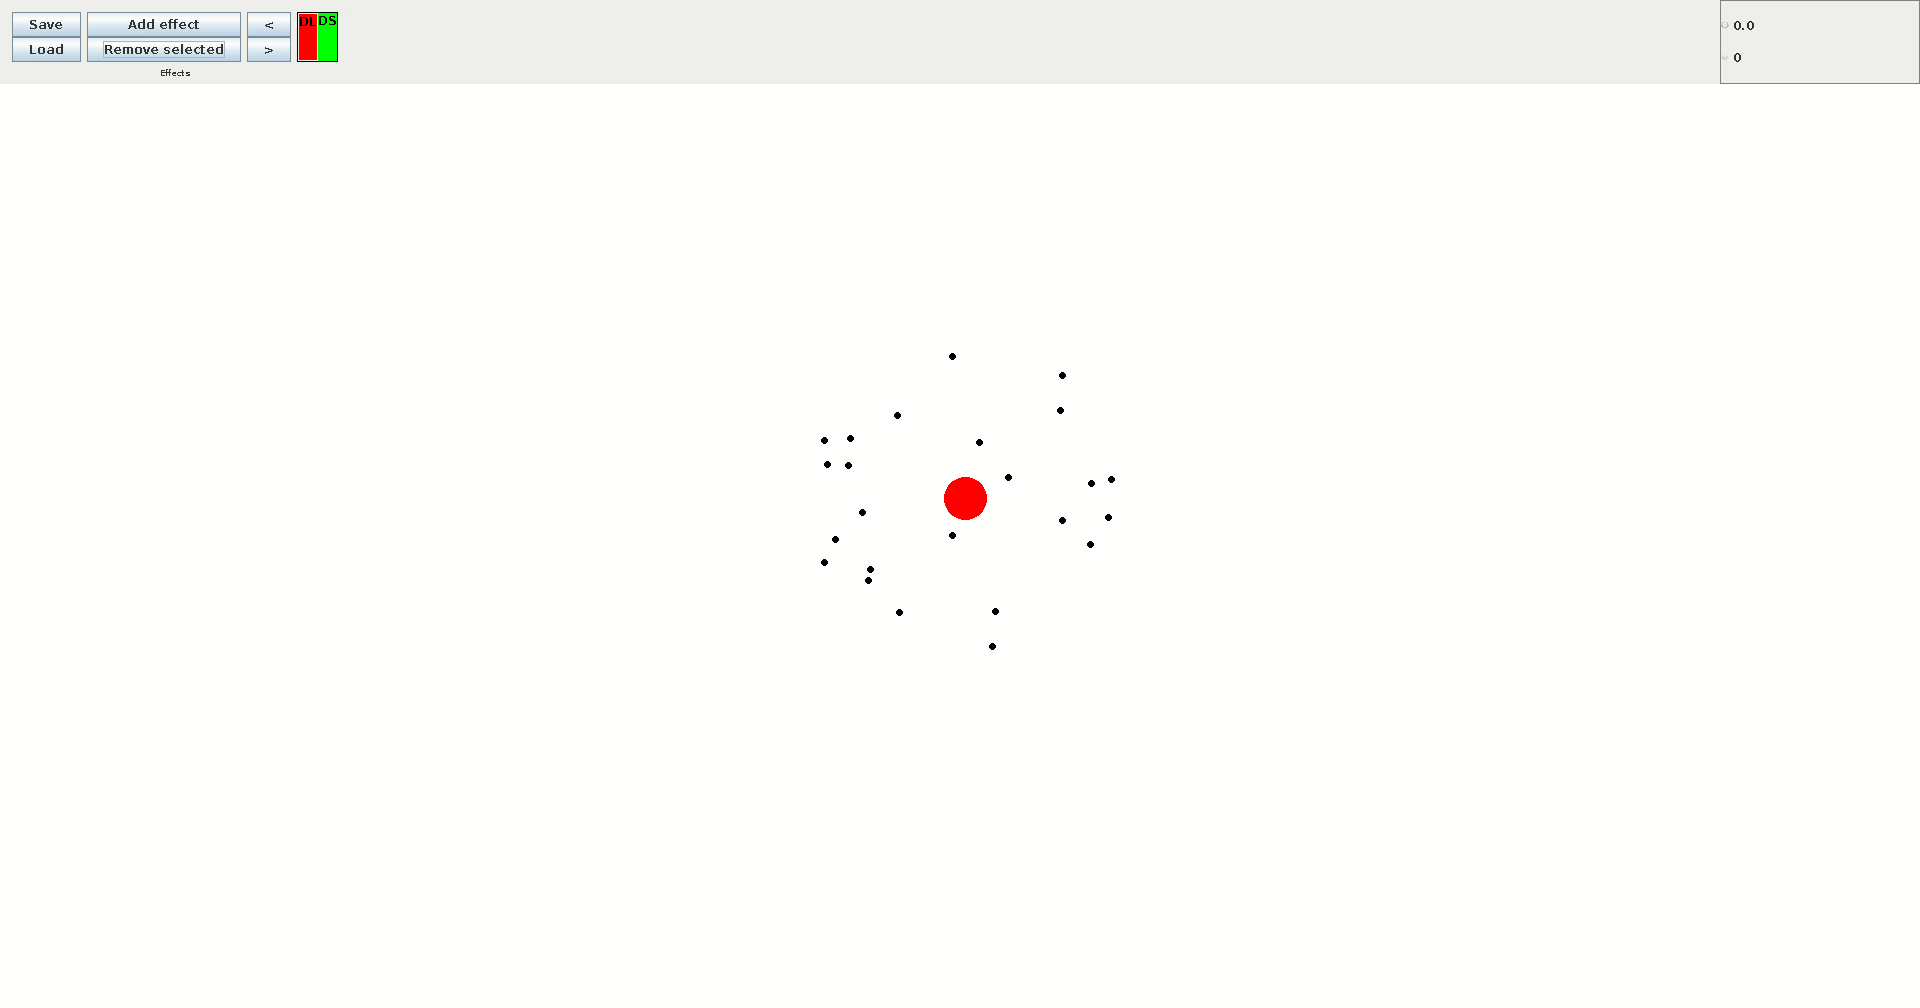
\includegraphics[width=\textwidth]{immagini/casi-studio/influence-without-groups-begin.png}
    \end{subfigure}
    \hfill
    \begin{subfigure}[b]{0.75\textwidth}
        \centering
        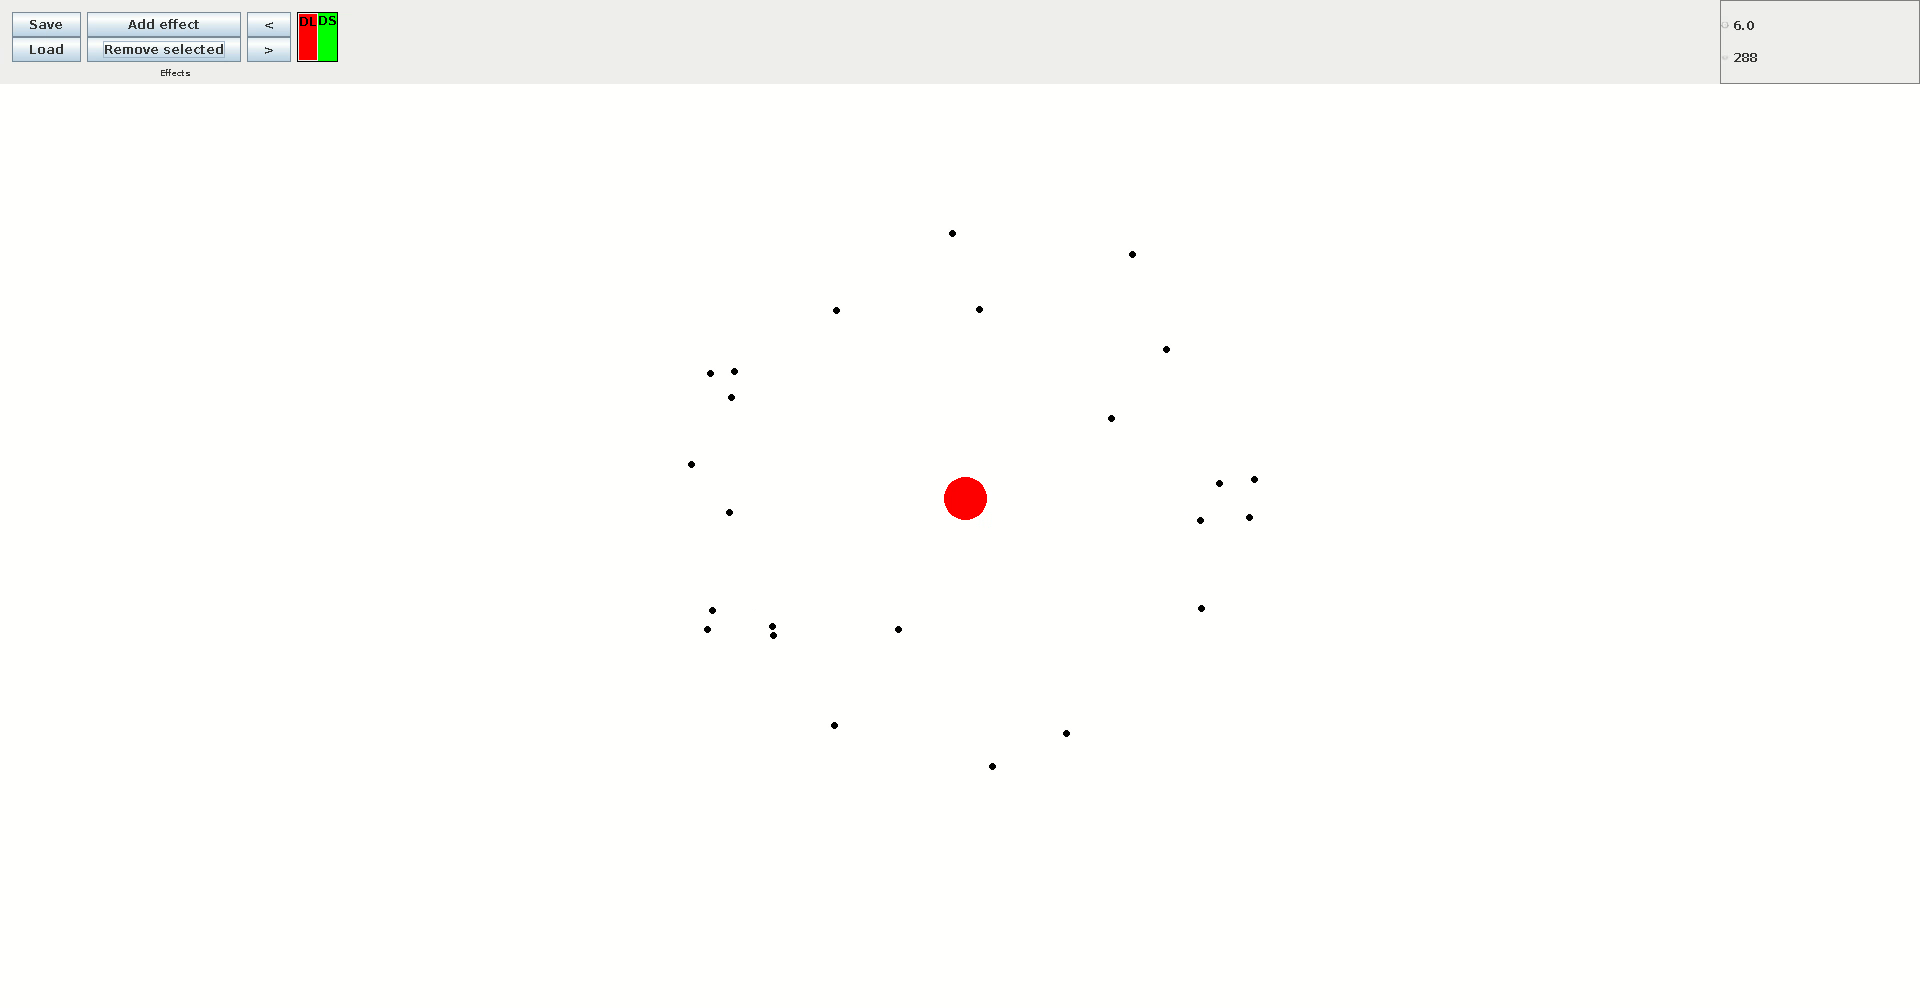
\includegraphics[width=\textwidth]{immagini/casi-studio/influence-without-groups-during.png}
    \end{subfigure}
    \hfill
    \begin{subfigure}[b]{0.75\textwidth}
        \centering
        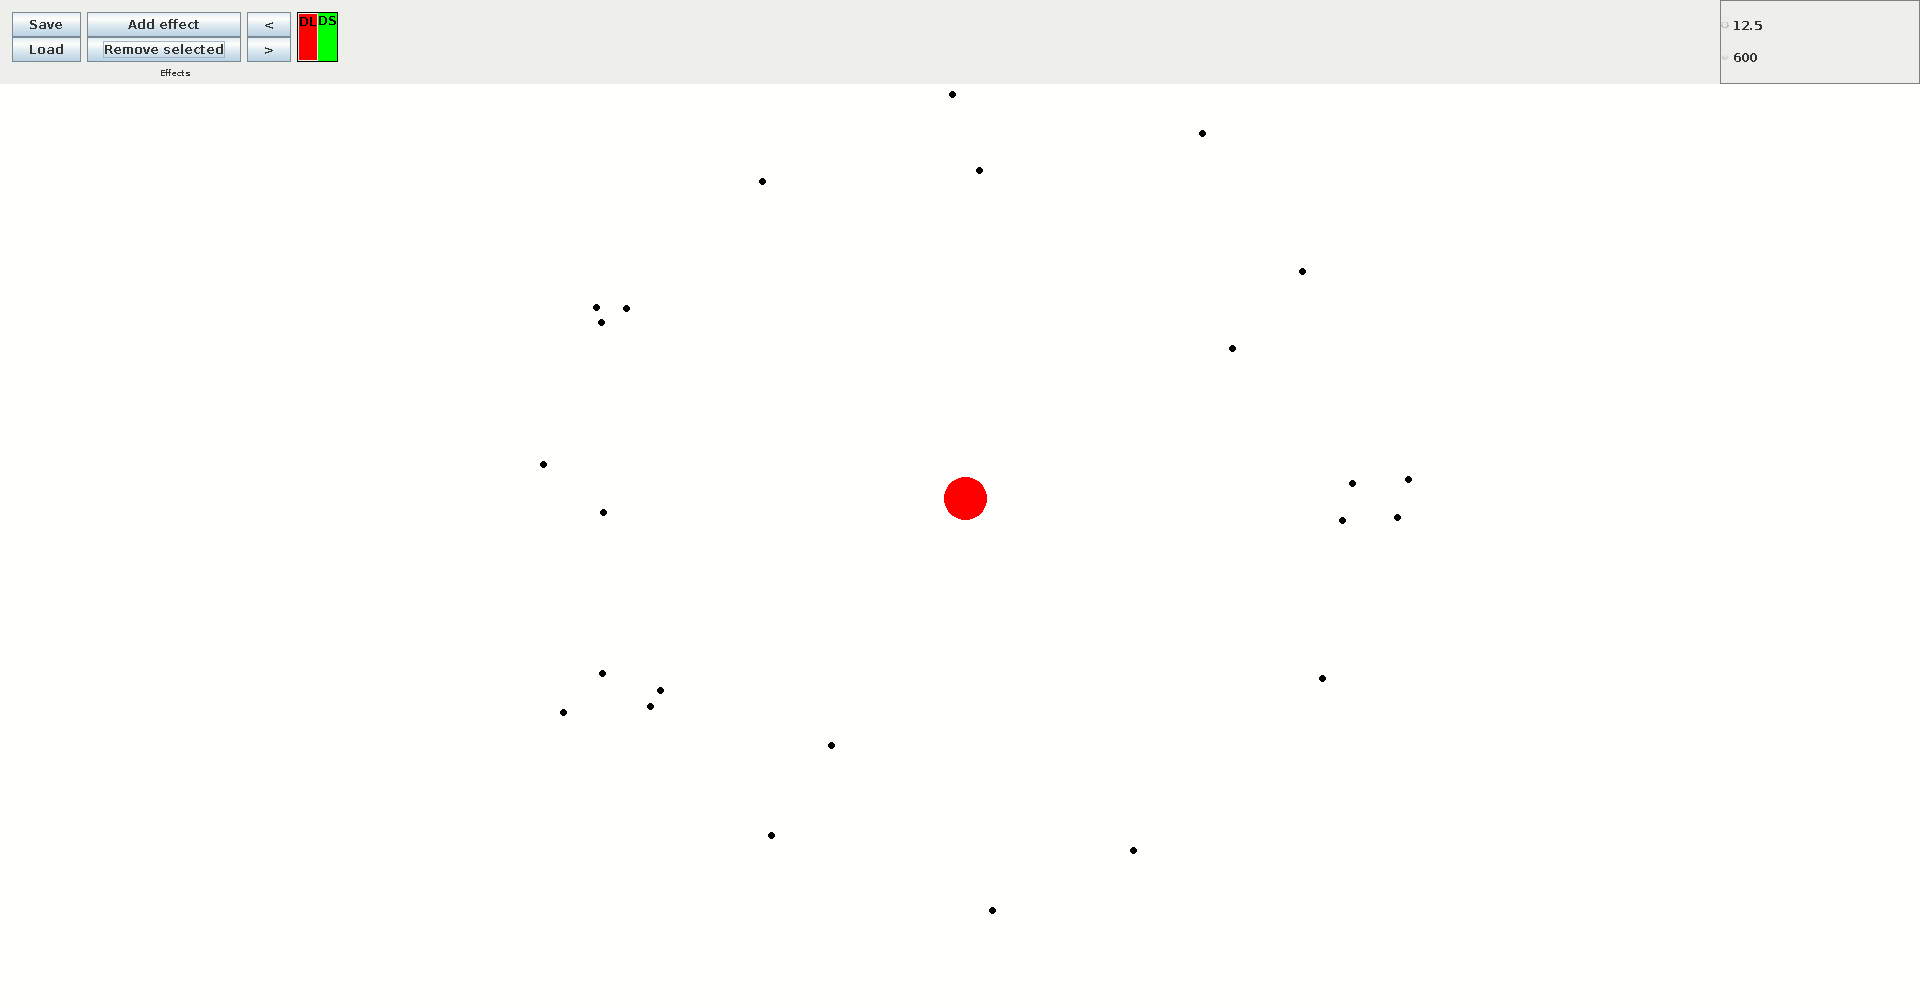
\includegraphics[width=\textwidth]{immagini/casi-studio/influence-without-groups-end.png}
    \end{subfigure}
    \caption{Fotogrammi salienti della simulazione sull'influenza del gruppo considerando pedoni solitari; è possibile notare come essi, pensando solo alla propria incolumità, si limitino a fuggire dalla zona di pericolo.}
    \label{fig:influence-without-groups}
\end{figure}

\begin{figure}
    \centering
    \begin{subfigure}[b]{0.75\textwidth}
        \centering
        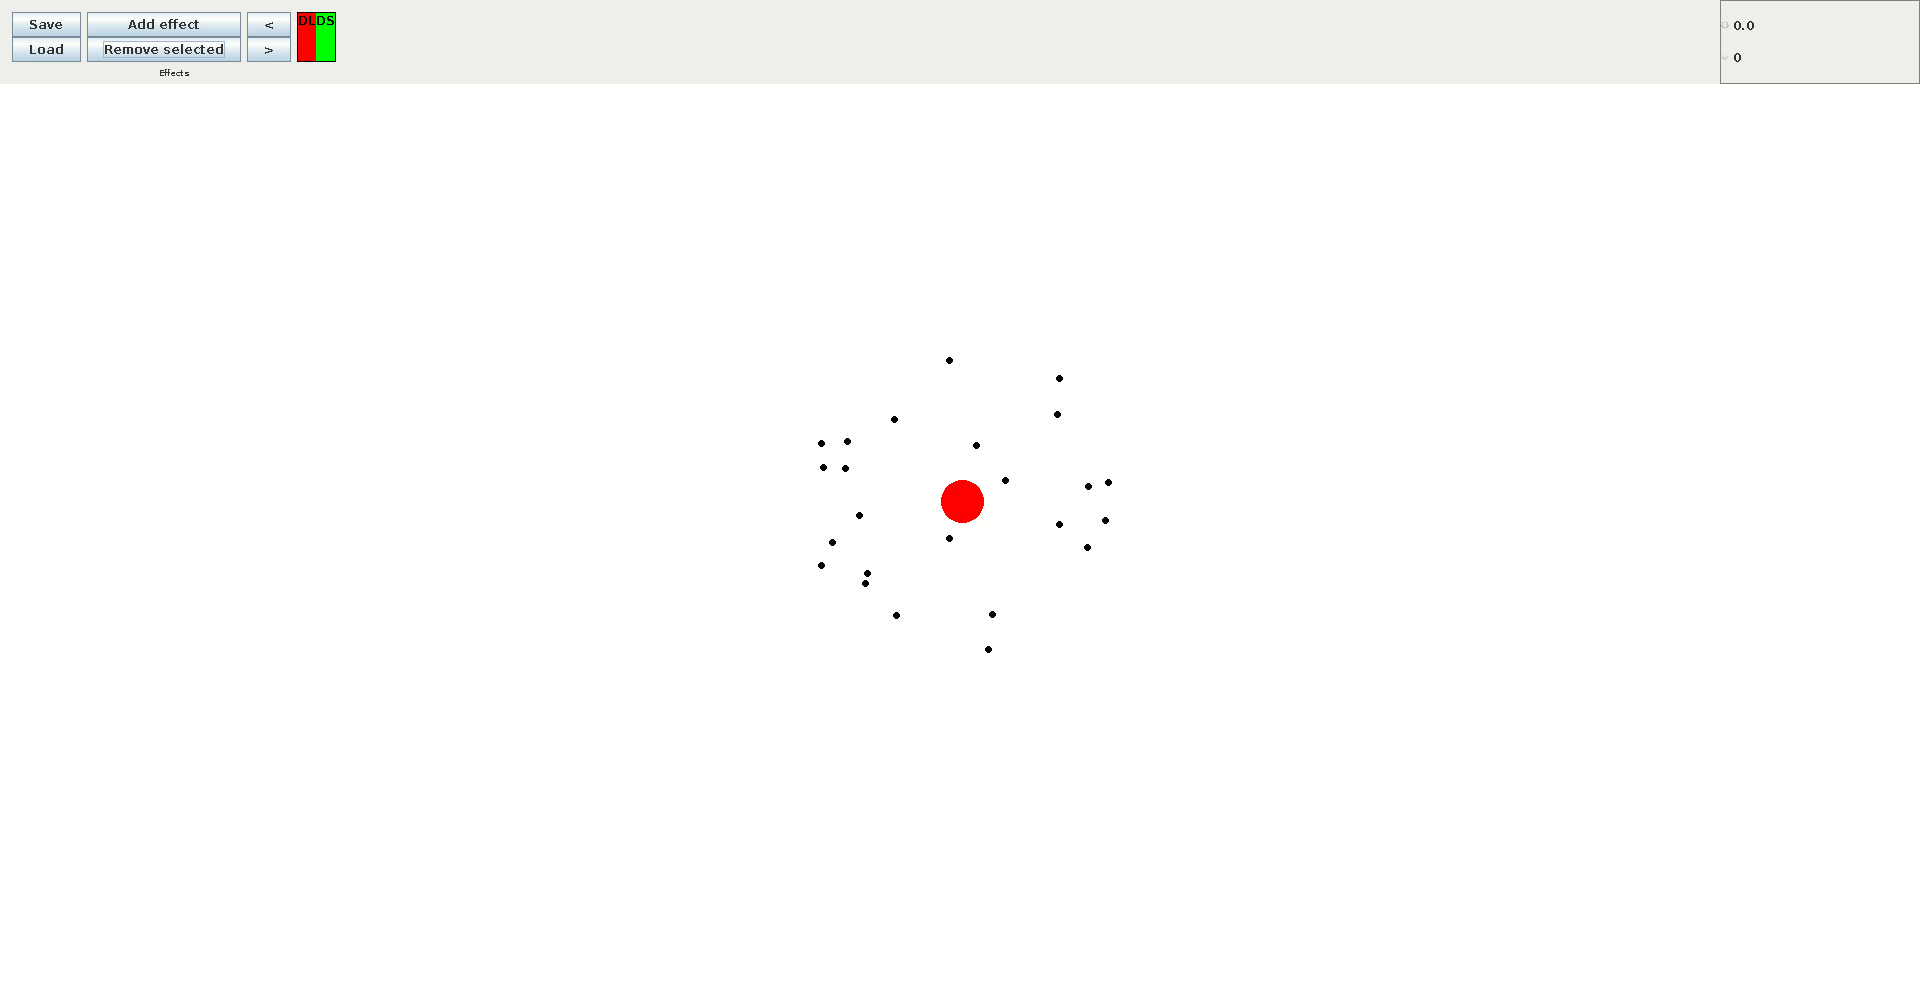
\includegraphics[width=\textwidth]{immagini/casi-studio/influence-with-groups-begin.png}
    \end{subfigure}
    \hfill
    \begin{subfigure}[b]{0.75\textwidth}
        \centering
        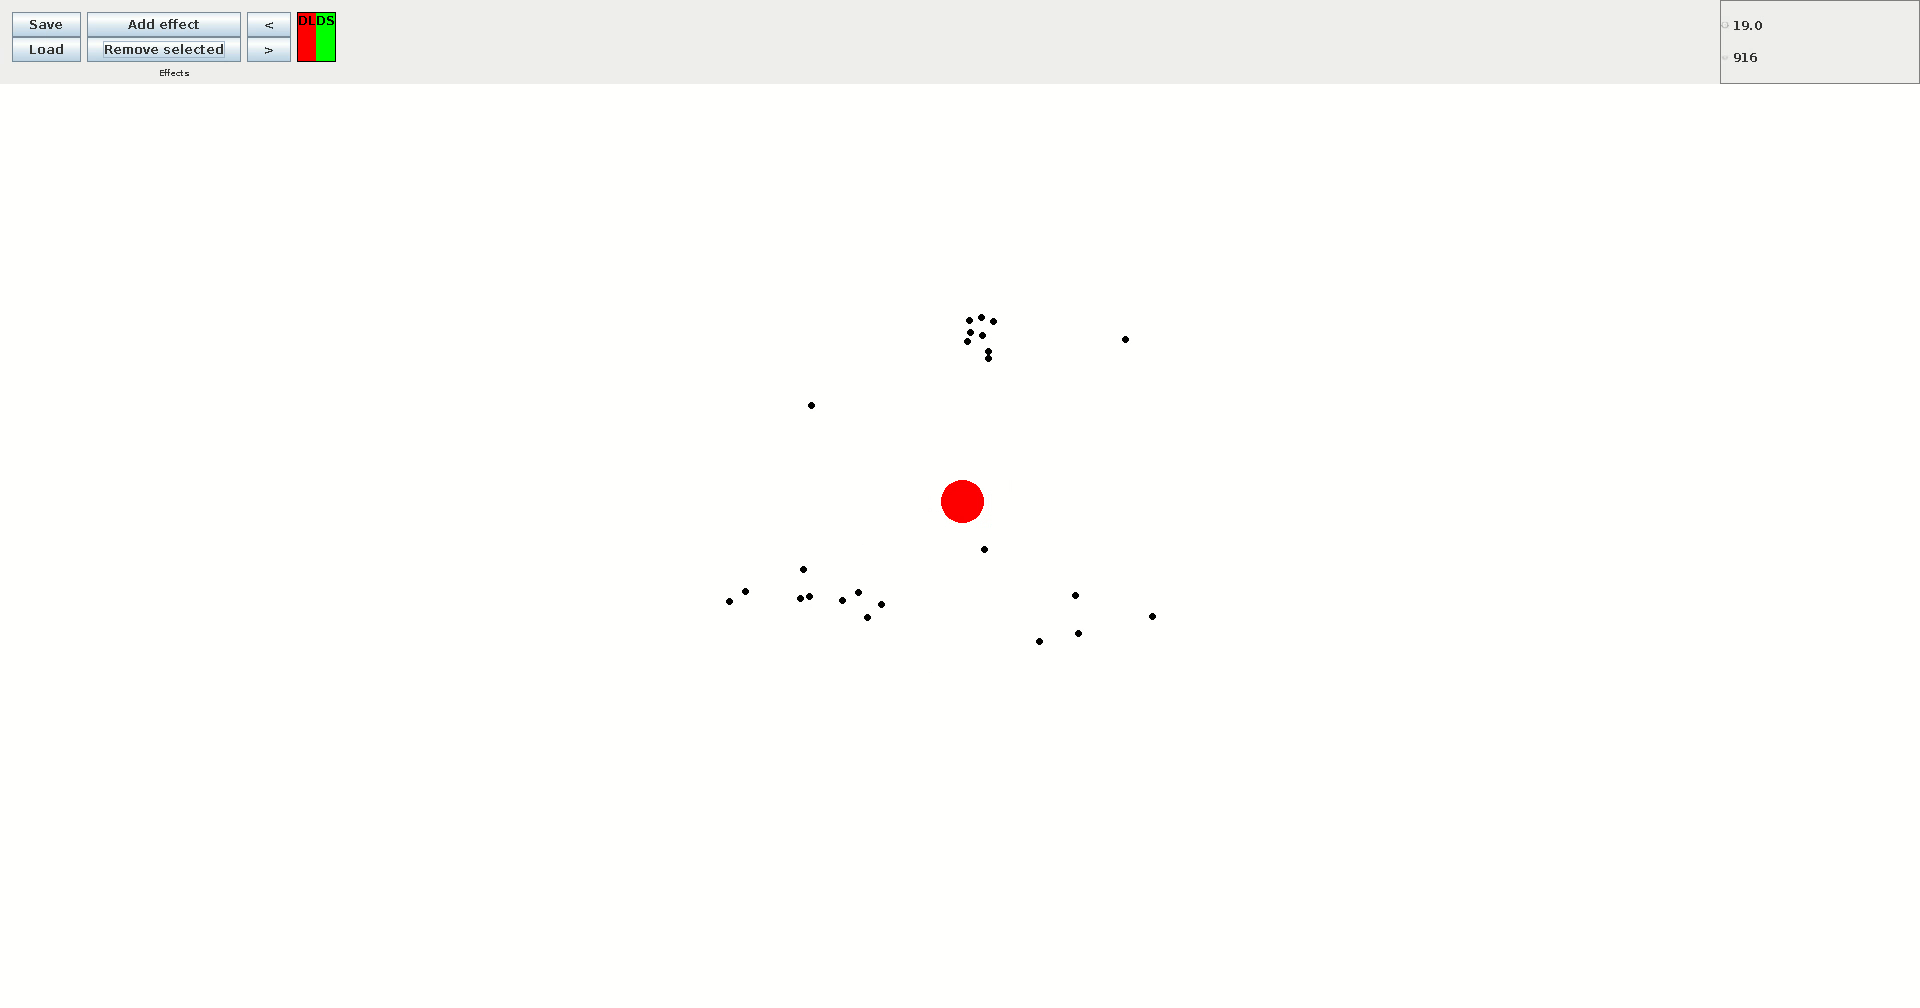
\includegraphics[width=\textwidth]{immagini/casi-studio/influence-with-groups-during.png}
    \end{subfigure}
    \hfill
    \begin{subfigure}[b]{0.75\textwidth}
        \centering
        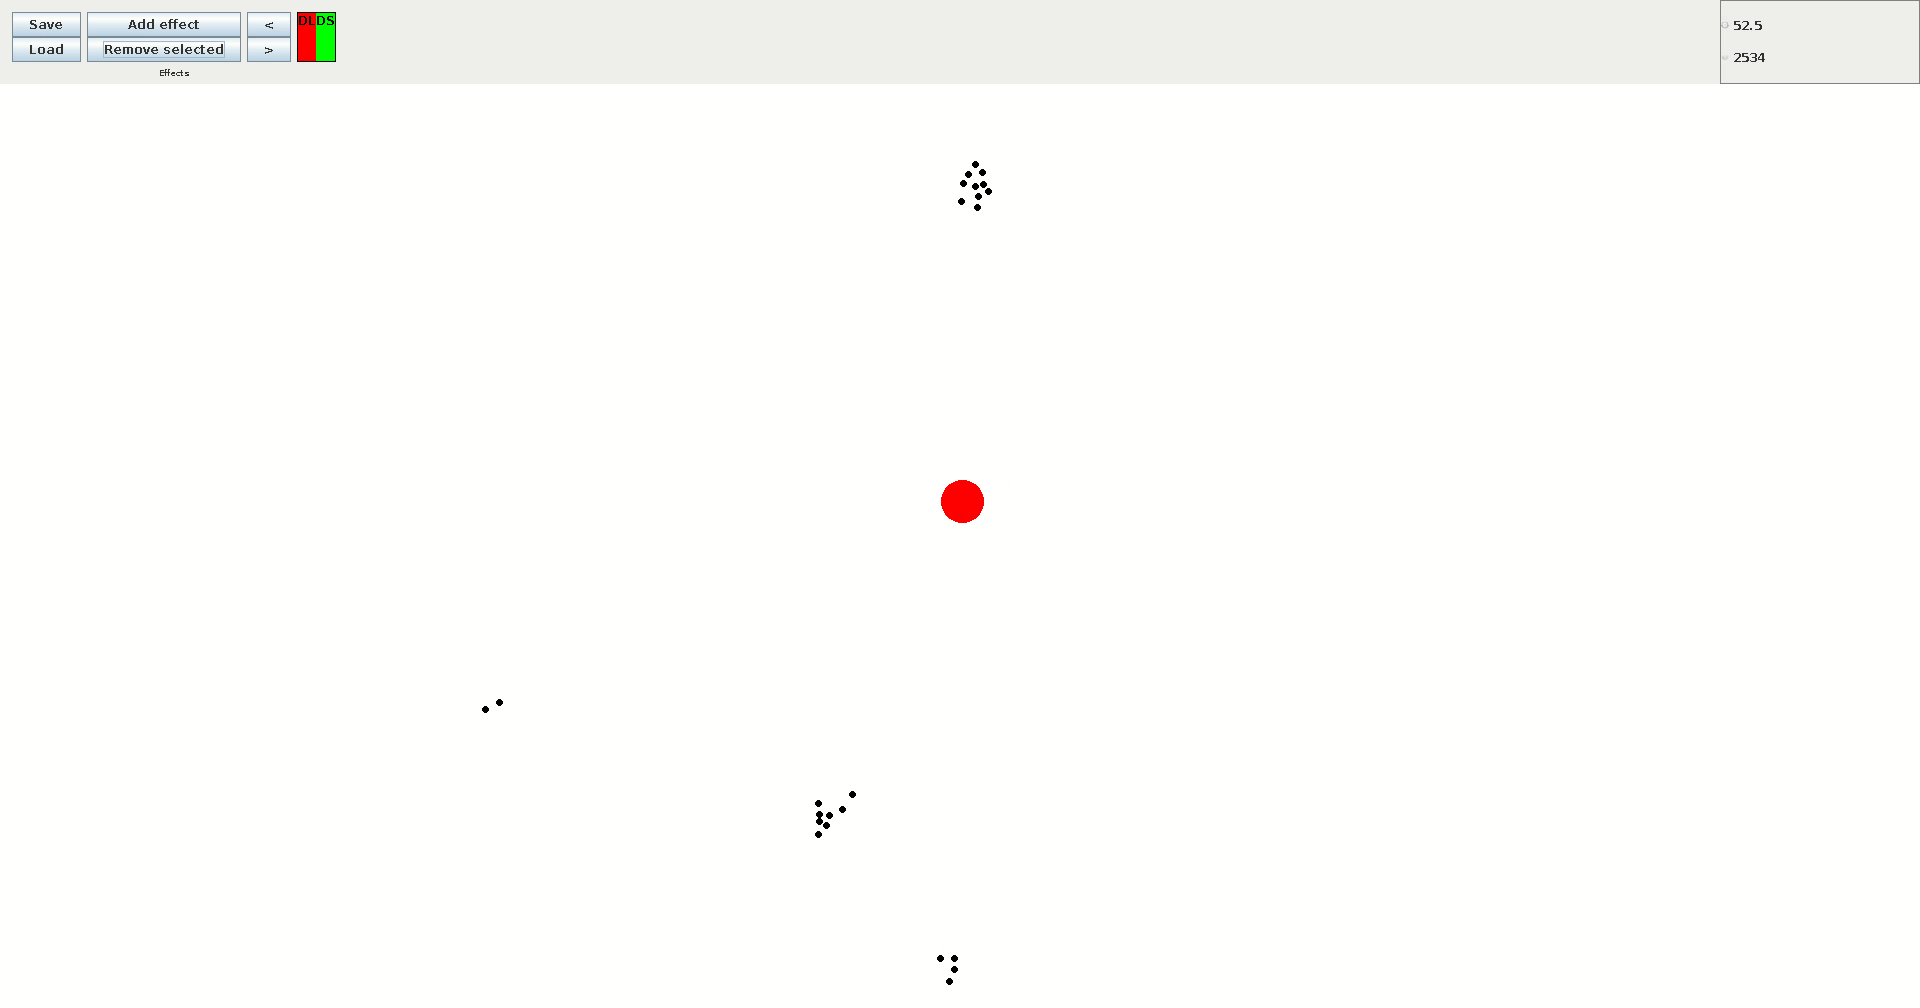
\includegraphics[width=\textwidth]{immagini/casi-studio/influence-with-groups-end.png}
    \end{subfigure}
    \caption{Fotogrammi salienti della simulazione sull'influenza del gruppo considerando quattro insiemi di amici; prima di allontanarsi dalla zona di pericolo, i pedoni cercano di riunirsi con tutti gli altri membri del loro stesso gruppo.}
    \label{fig:influence-with-groups}
\end{figure}
\section{Contagio sociale}
Le scelte di un agente possono riflettere, oltre al proprio, anche lo stato d'animo degli altri soggetti che popolano l'ambiente di interesse. Ogni atteggiamento che scaturisce da una persona può essere, in positivo quanto in negativo, causa della medesima risposta anche in un'altra. \newline
Alla base di questo principio, c'è il già citato meccanismo del contagio sociale, che ha nella trasmissione della paura il suo più lampante esempio. Vedendo un intero gruppo scappare terrorizzato, infatti, la reazione spontanea per un essere umano è quella di fare altrettanto, anche se non si è riscontrata presenza concreta del pericolo.

\subsection{Descrizione della simulazione}
In un ambiente euclideo continuo ed illimitato, vengono definite una zona di sicurezza ed una di pericolo da parti opposte e sono caricati, nello spazio compreso tra esse, due raggruppamenti di pedoni rispettivamente costituiti da 75 e 25 persone. \newline 
Mentre il gruppo più numeroso, costituito da pedoni cognitivi, viene posizionato in prossimità del pericolo, quello meno numeroso è collocato a debita distanza da esso. Nonostante la distanza, la traiettoria da seguire per raggiungere il più velocemente possibile la zona di sicurezza è la stessa per entrambi. \newline
La simulazione è stata eseguita in due casi, differenziando la tipologia di pedone utilizzata per il gruppo da 25: eterogeneo nella prima, cognitivo nella seconda.

\subsection{Risultati ottenuti}
Come è possibile osservare dai momenti significativi raccolti in figura \ref{fig:social-contagion-not-cognitive}, i pedoni eterogenei, trovandosi lontani e non potendo percepire direttamente il pericolo, rimangono al loro posto per tutto il decorrere della simulazione e osservano indifferenti il gruppo costituito dai 75 agenti cognitivi passargli vicino nell'intento di raggiungere la zona di sicurezza. \newline
Diversamente, valutando la situazione negli stessi istanti temporali, ma in presenza di soli agenti cognitivi (figura \ref{fig:social-contagion-cognitive}), possiamo notare come progressivamente anche il secondo gruppo, impaurito dallo stato emotivo dei pedoni del primo, inizi a scappare nella stessa direzione. 

\begin{figure}
    \centering
    \begin{subfigure}[b]{0.75\textwidth}
        \centering
        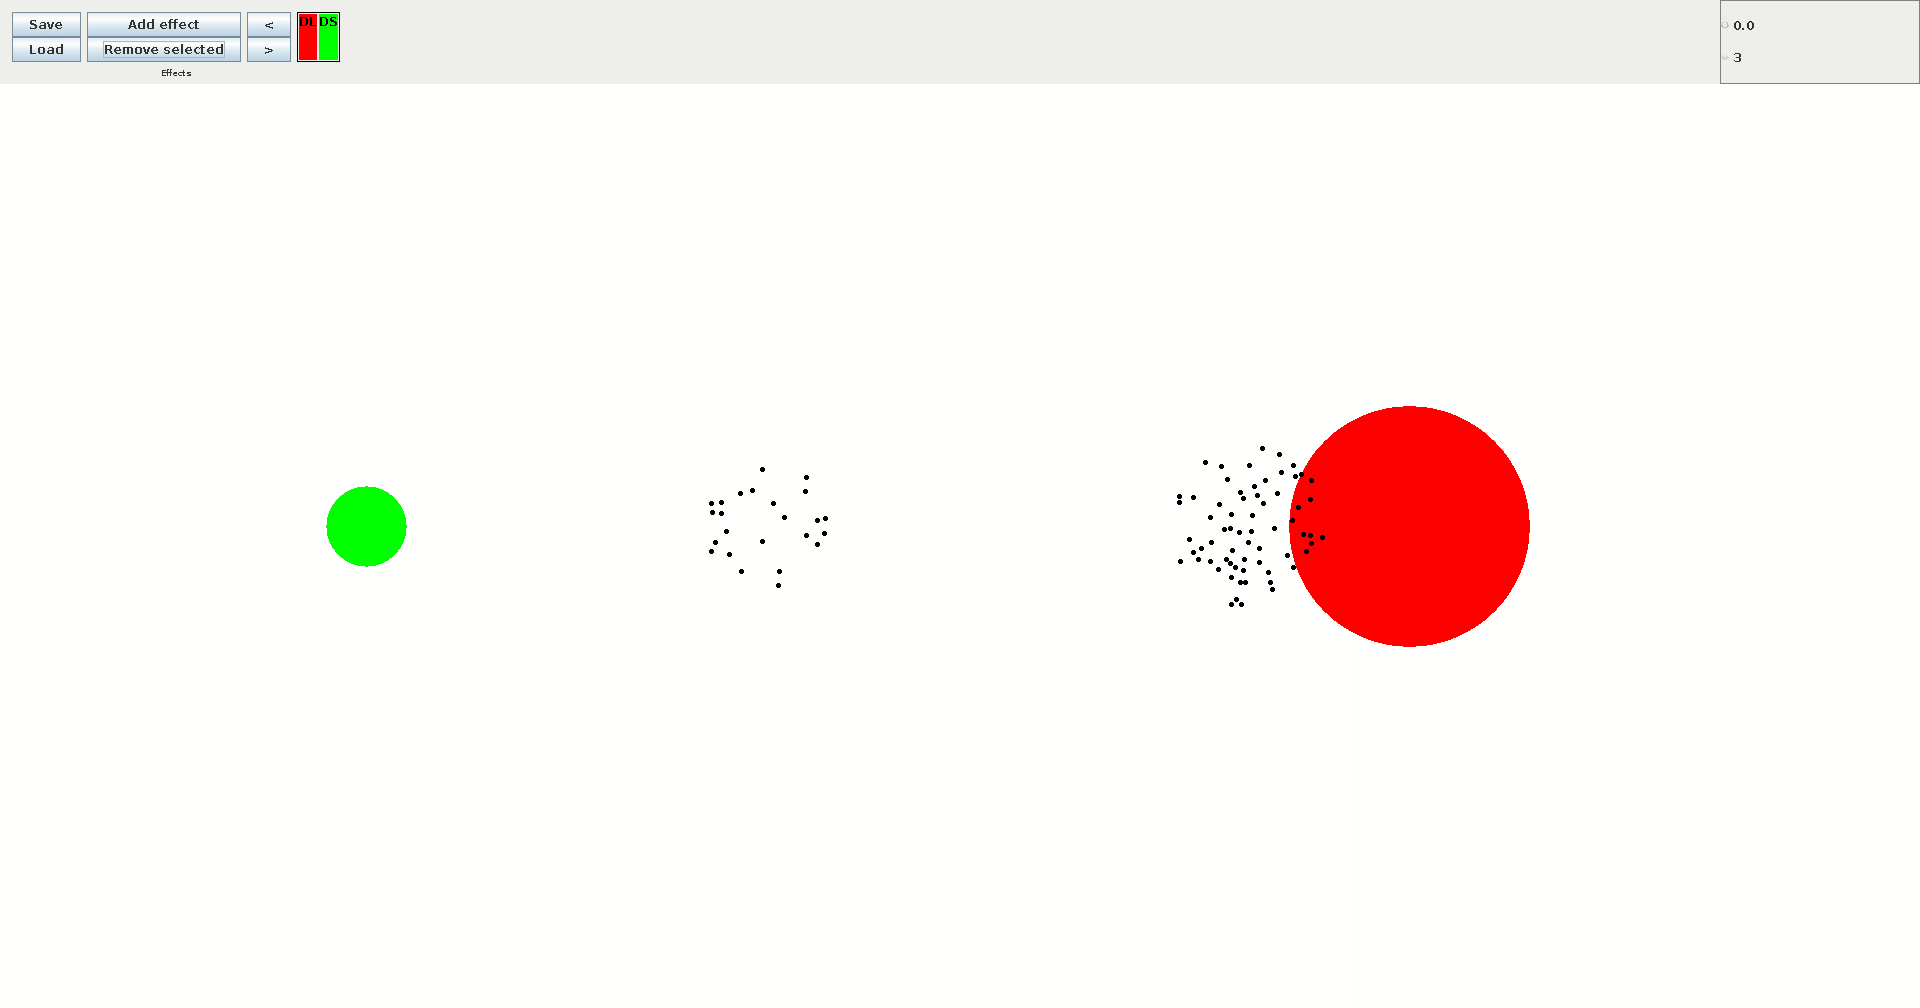
\includegraphics[width=\textwidth]{immagini/casi-studio/social-contagion-not-cognitive-begin.png}
    \end{subfigure}
    \hfill
    \begin{subfigure}[b]{0.75\textwidth}
        \centering
        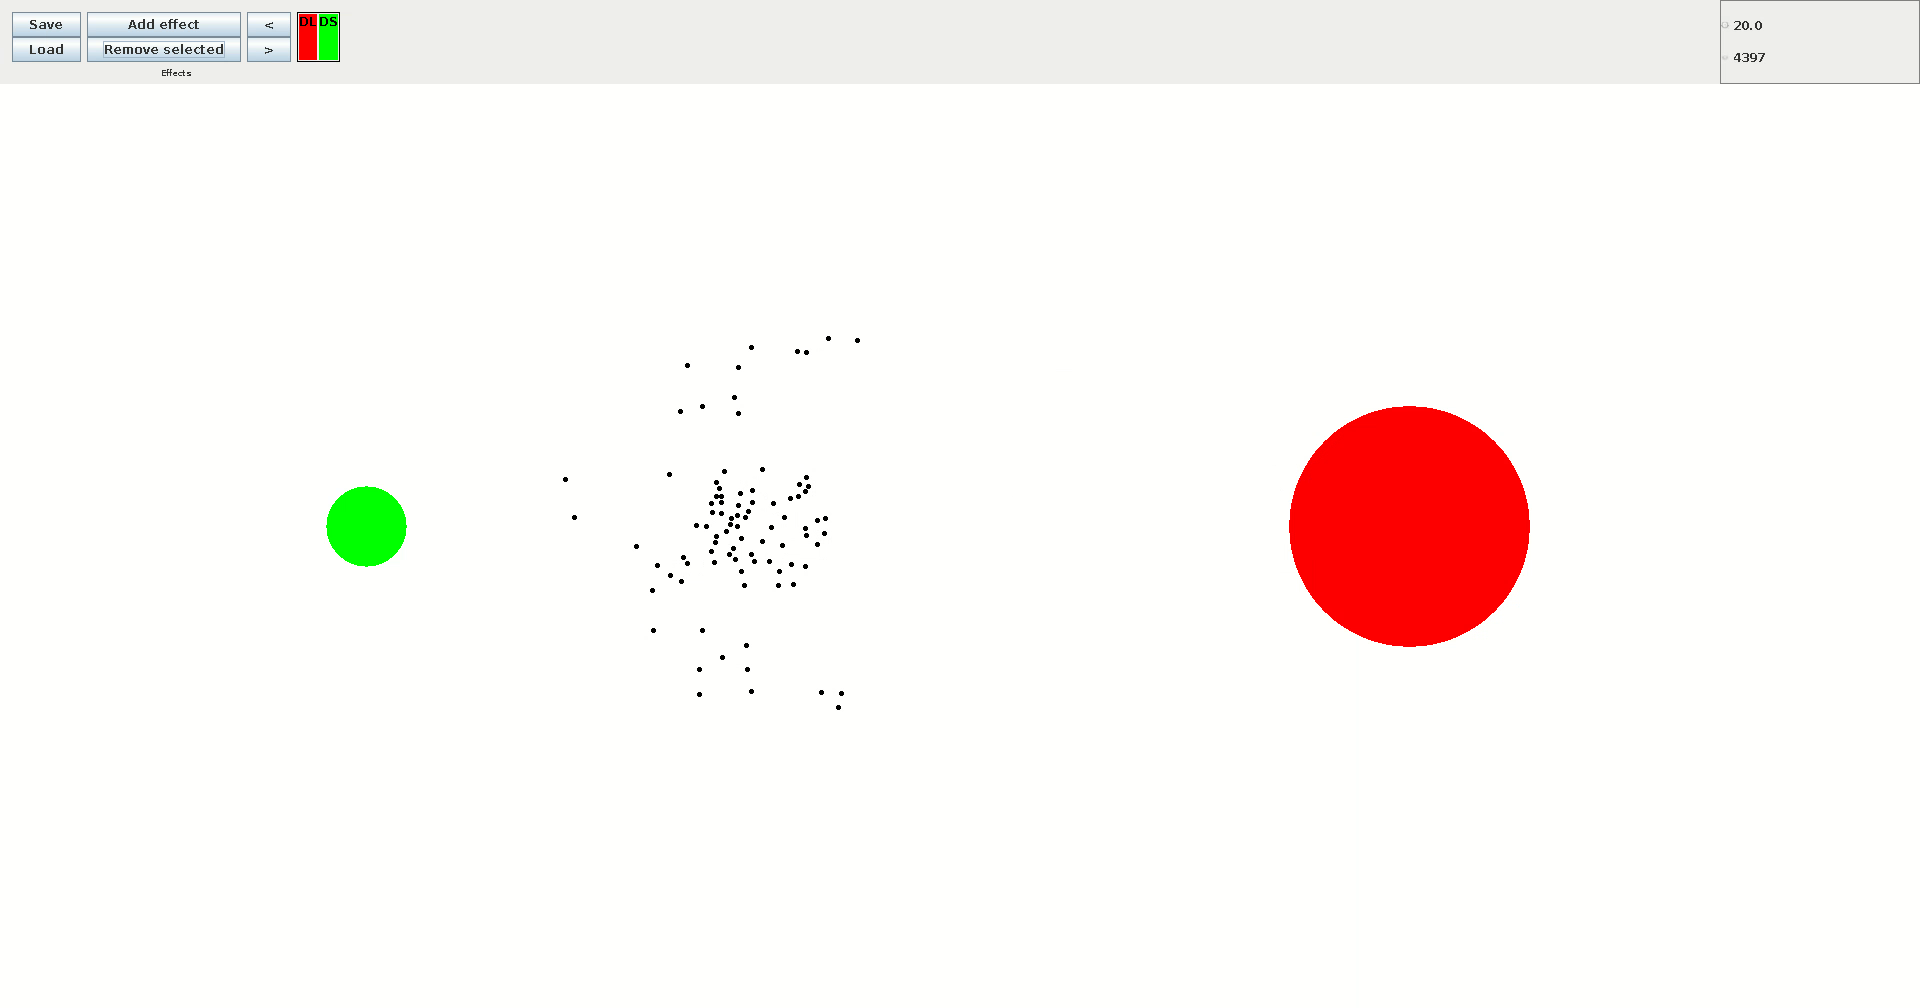
\includegraphics[width=\textwidth]{immagini/casi-studio/social-contagion-not-cognitive-during.png}
    \end{subfigure}
    \hfill
    \begin{subfigure}[b]{0.75\textwidth}
        \centering
        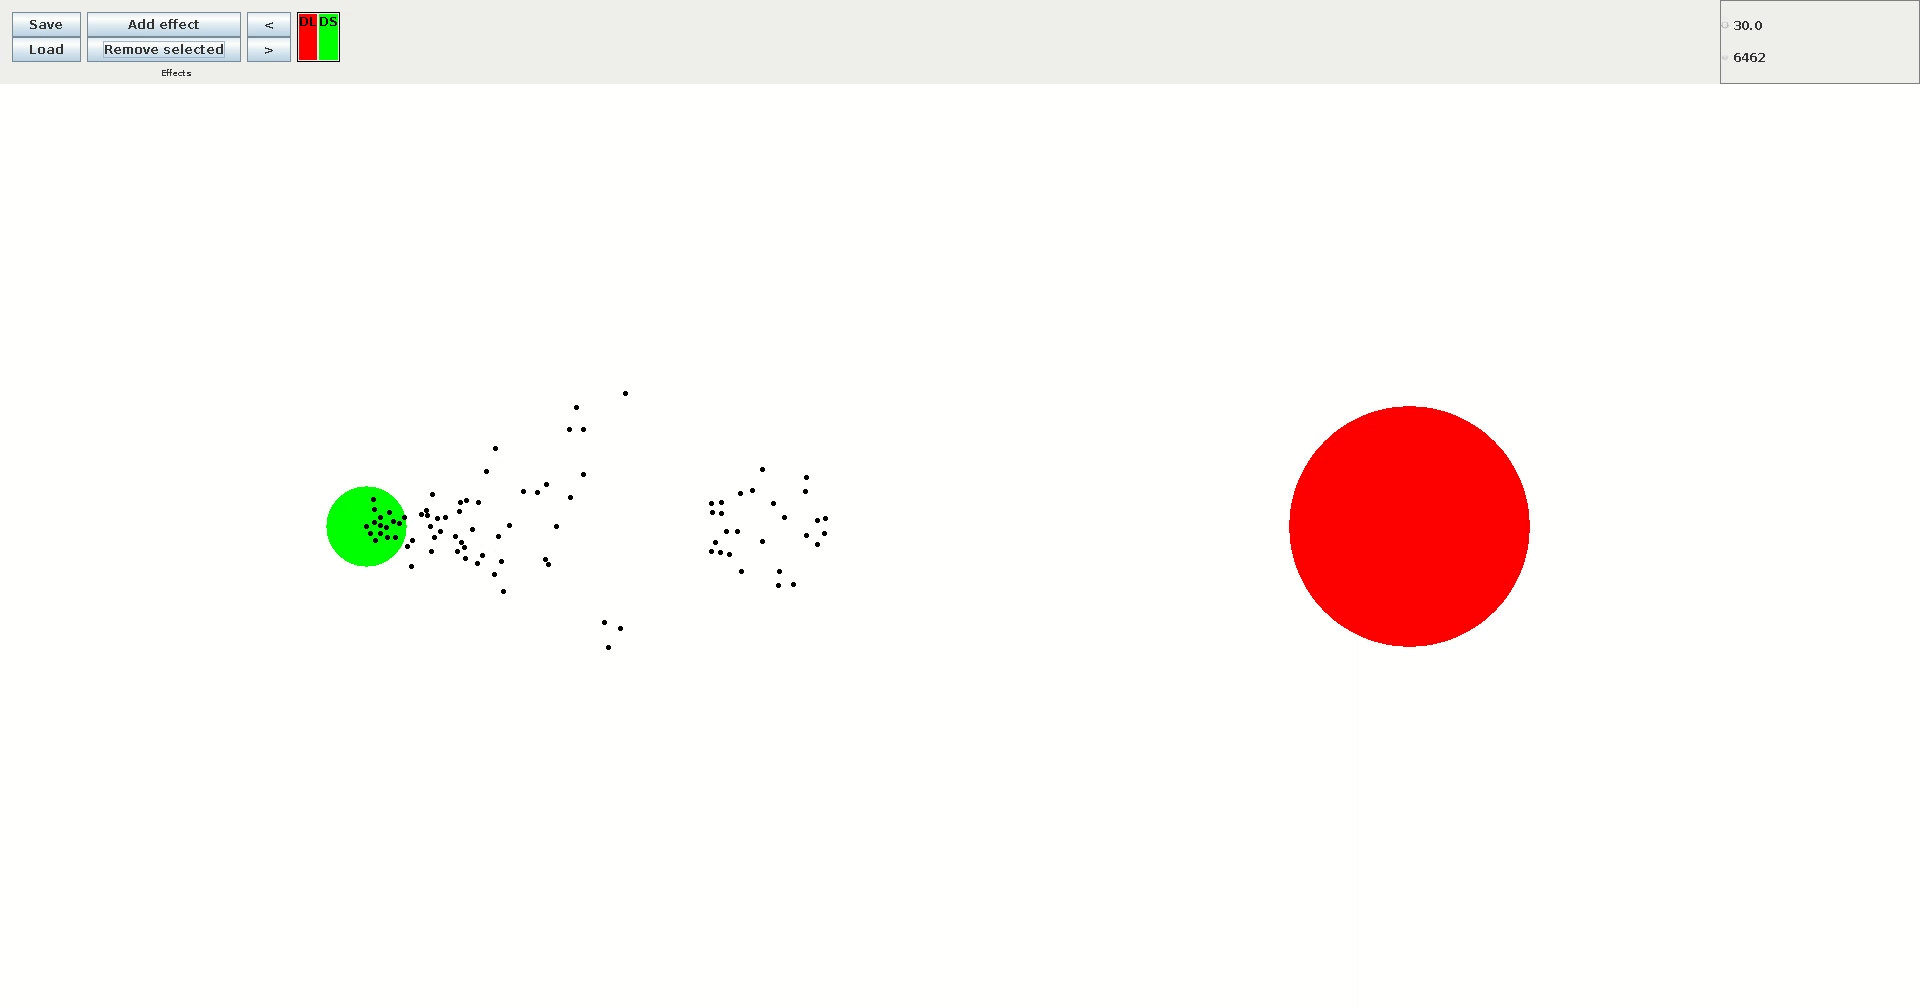
\includegraphics[width=\textwidth]{immagini/casi-studio/social-contagion-not-cognitive-end.png}
    \end{subfigure}
    \caption{Fotogrammi salienti della simulazione sul contagio sociale in presenza di pedoni non cognitivi; non avendo delle caratteristiche emotive e non potendo quindi percepire il panico degli agenti nel gruppo di destra, essi rimangono al loro posto.}
    \label{fig:social-contagion-not-cognitive}
\end{figure}

\begin{figure}
    \centering
    \begin{subfigure}[b]{0.75\textwidth}
        \centering
        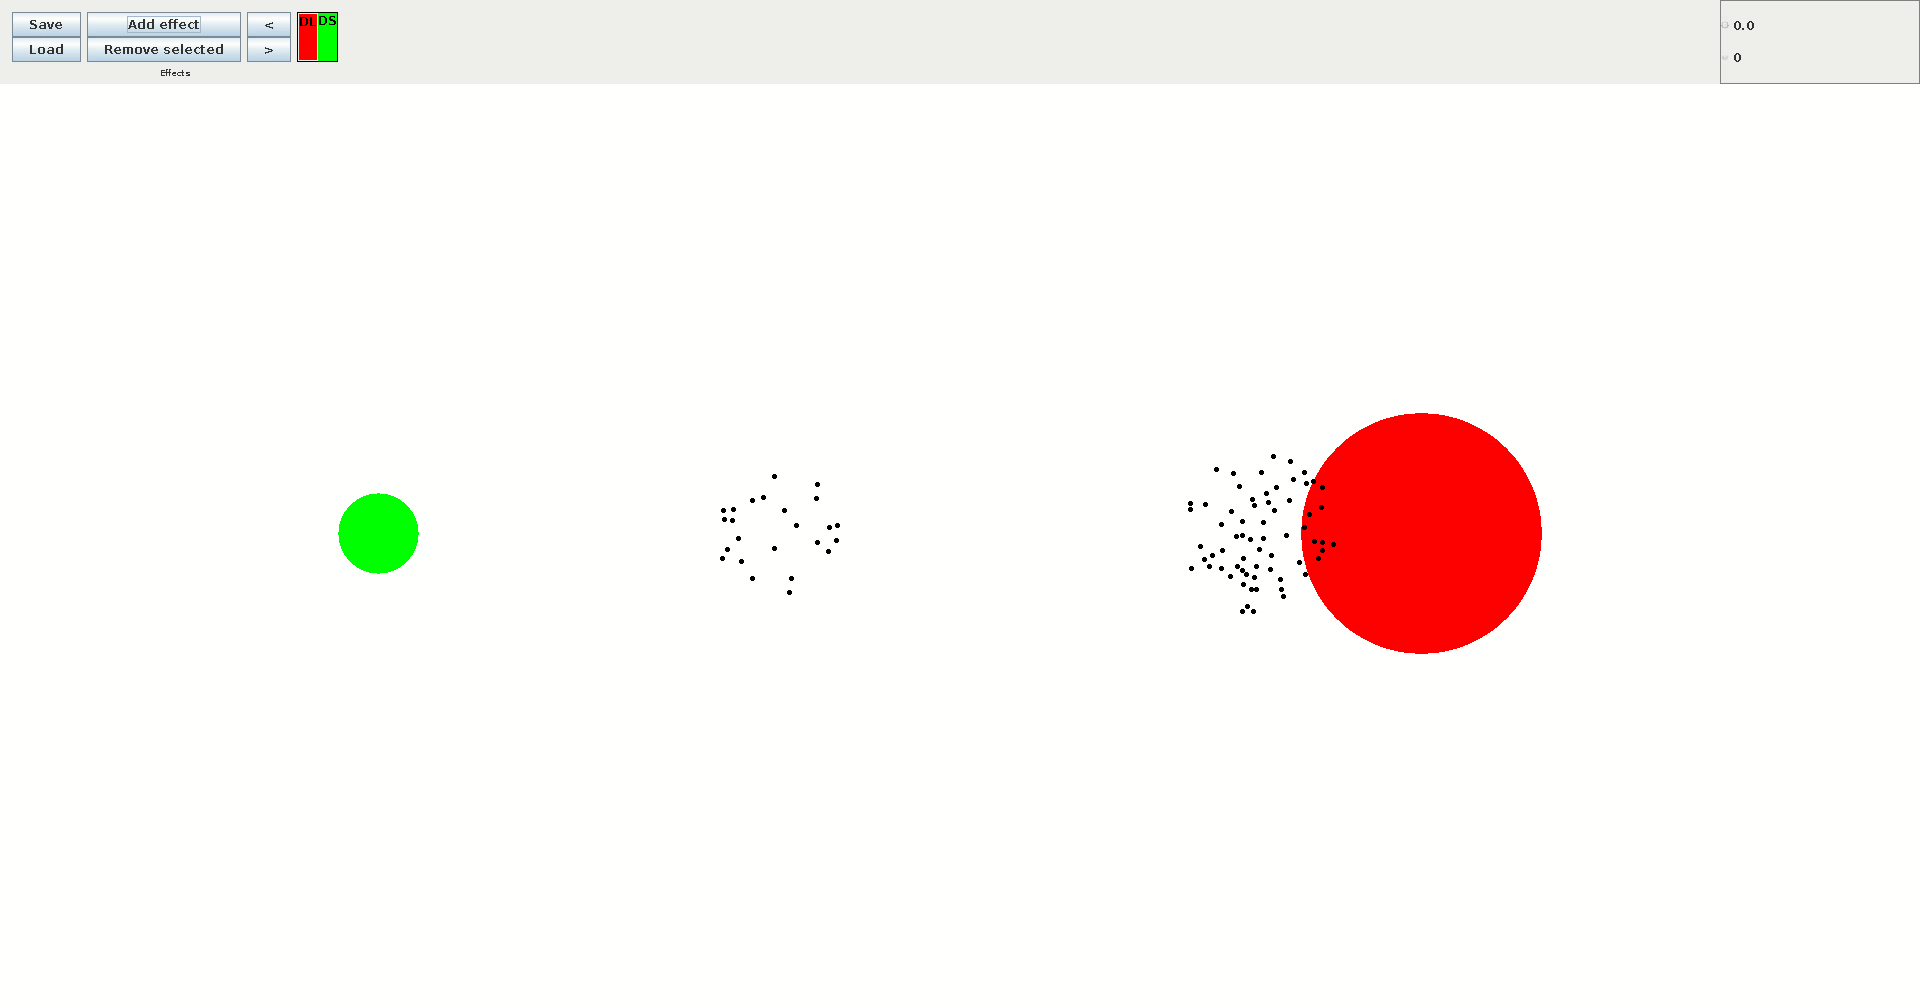
\includegraphics[width=\textwidth]{immagini/casi-studio/social-contagion-cognitive-begin.png}
    \end{subfigure}
    \hfill
    \begin{subfigure}[b]{0.75\textwidth}
        \centering
        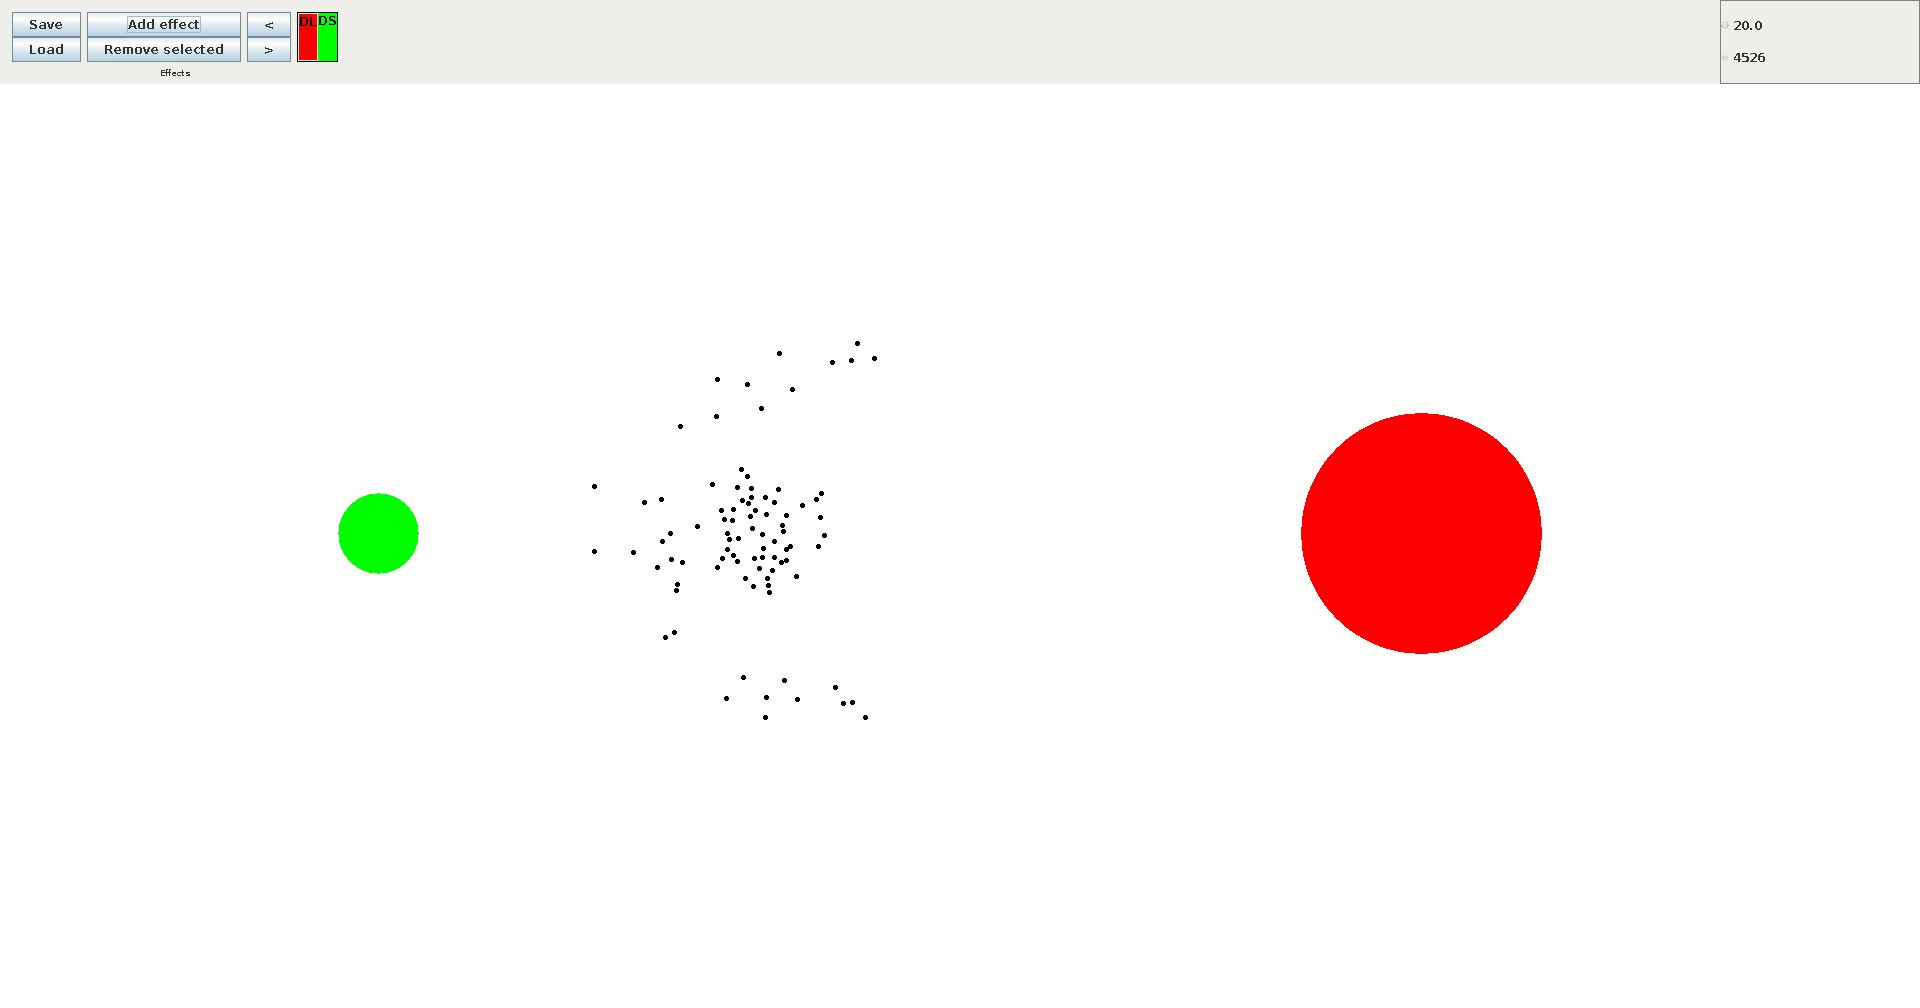
\includegraphics[width=\textwidth]{immagini/casi-studio/social-contagion-cognitive-during.png}
    \end{subfigure}
    \hfill
    \begin{subfigure}[b]{0.75\textwidth}
        \centering
        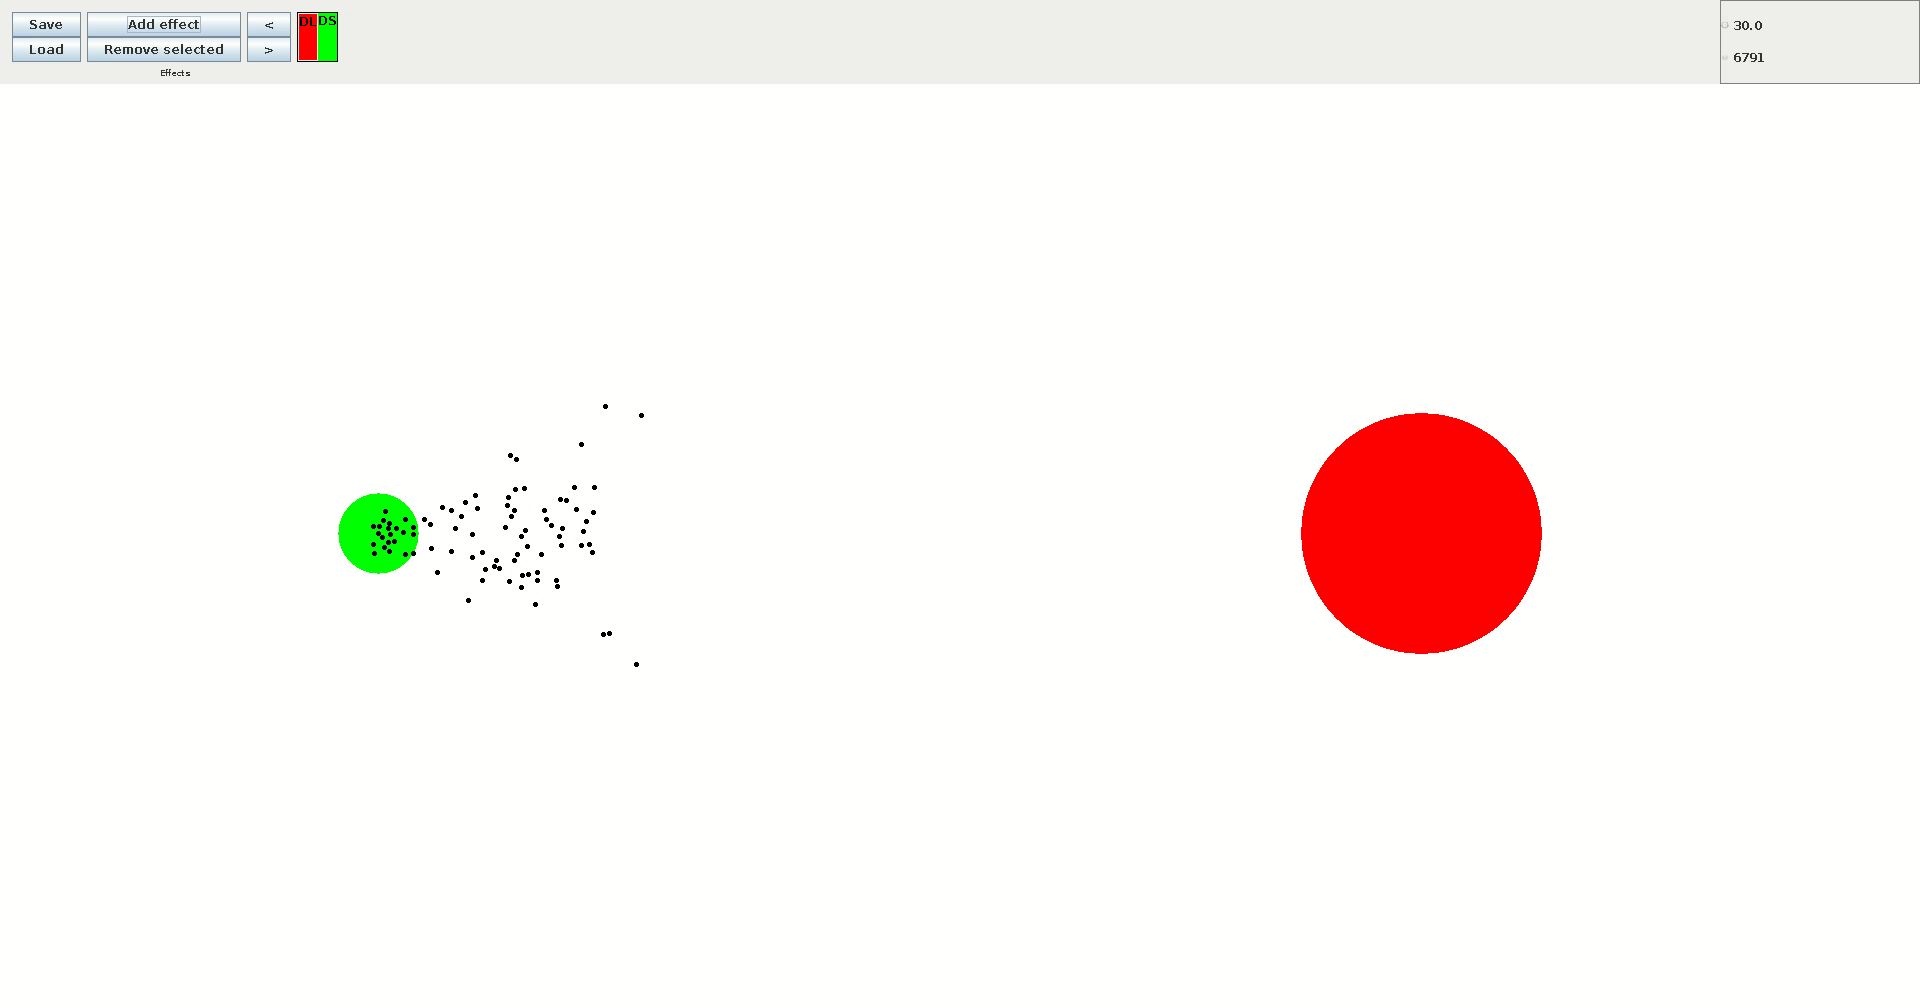
\includegraphics[width=\textwidth]{immagini/casi-studio/social-contagion-cognitive-end.png}
    \end{subfigure}
    \caption{Fotogrammi salienti della simulazione sul contagio sociale in presenza di pedoni cognitivi; il fenomeno della trasmissione del panico nel momento in cui i due gruppi si incrociano, porta gli agenti precedentemente fermi ad iniziare a fuggire.}
    \label{fig:social-contagion-cognitive}
\end{figure}
\section{Scelta dell'uscita}
Un'ambientazione realistica presenta tipicamente molteplici elementi, che contribuiscono ad aumentare la complessità della situazione da analizzare. \newline 
Ad esempio, pensando alla planimetria di un edificio, è inusuale che vi sia una sola uscita, in quanto una scelta del genere comporterebbe problemi sia dal punto di vista logistico sia da quello della sicurezza. \newline
Per determinare i probabili movimenti di una folla in uno scenario contraddistinto da più punti di interesse aventi lo stesso scopo, è necessario scegliere con cura la strategia da utilizzare per la combinazione delle varie forze in gioco, altrimenti si rischia di ottenere simulazioni poco attendibili.

\subsection{Descrizione della simulazione}
Lo scenario utilizzato è molto simile a quello impiegato nelle simulazioni del modello IMPACT: un ambiente limitato di dimensione quadrata con quattro uscite, al centro del quale è presente una zona di pericolo. Intorno ad essa, sono disposti casualmente 150 agenti cognitivi. \newline
In questo caso, non è possibile definire univocamente il movimento dei vari pedoni, in quanto, essendo presenti multiple uscite, non tutti hanno in comune lo stesso punto di arrivo. \newline
La stessa simulazione è stata ripetuta prima considerando come reazione responsabile del movimento il \texttt{BlendedSteering}, che utilizza la strategia basata sulla distanza, poi il \texttt{PrioritySteering}, che utilizza la strategia basata sulla massima vicinanza.

\subsection{Risultati ottenuti}
I momenti salienti in figura \ref{fig:multiple-exits-blended} dimostrano come l'utilizzo del \texttt{BlendedSteering} non sia adatto a descrivere la situazione e conduca a risultati inverosimili, dovuti al fatto che il pedone rimane perennemente indeciso su quale uscita scegliere in maniera particolare se si trova al centro della stanza, che è il luogo da cui dovrebbe avere più interesse a stare lontano. \newline
Ben diverso è il risultato nel caso si utilizzi il \texttt{PrioritySteering} (figura \ref{fig:multiple-exits-priority}), che determina un comportamento più simile a quello che si osserverebbe nella vita reale, contraddistinto da un iniziale allontanamento dal pericolo seguito dal raggiungimento dell'uscita più vicina.

\begin{figure}
    \centering
    \begin{subfigure}[b]{0.75\textwidth}
        \centering
        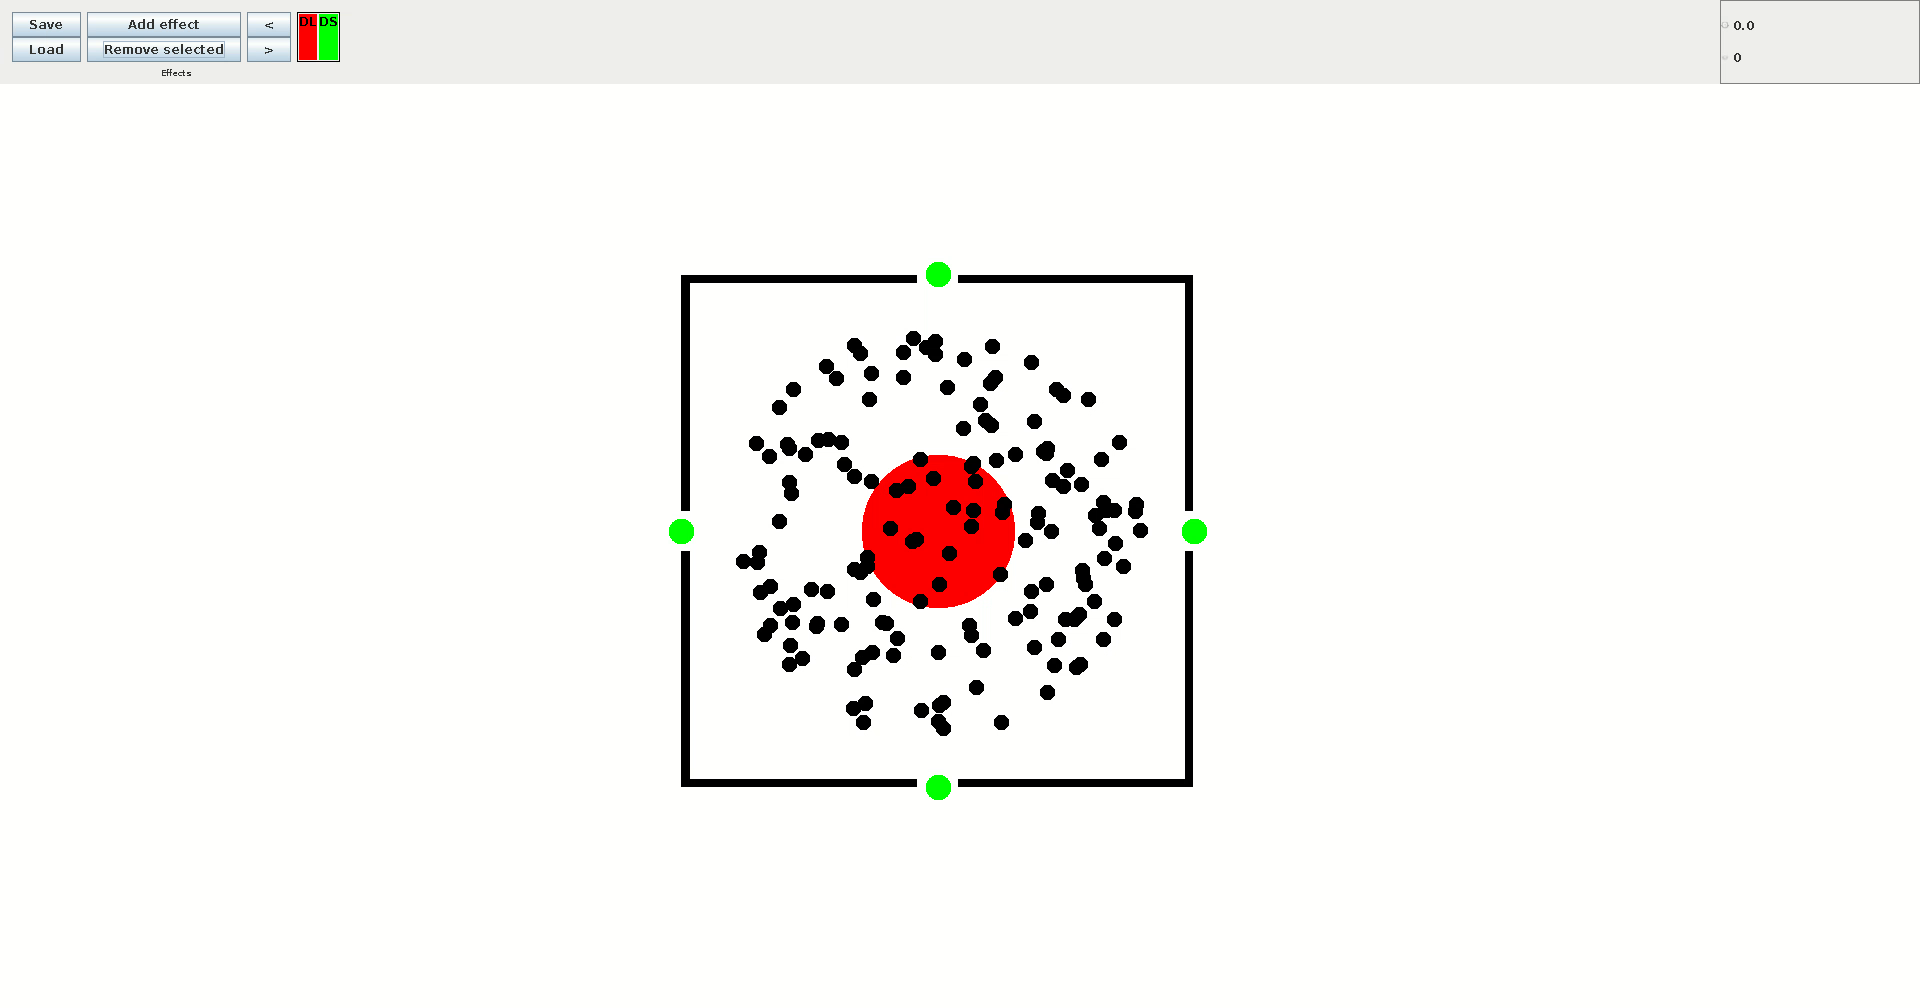
\includegraphics[width=\textwidth]{immagini/casi-studio/multiple-exits-blended-begin.png}
    \end{subfigure}
    \hfill
    \begin{subfigure}[b]{0.75\textwidth}
        \centering
        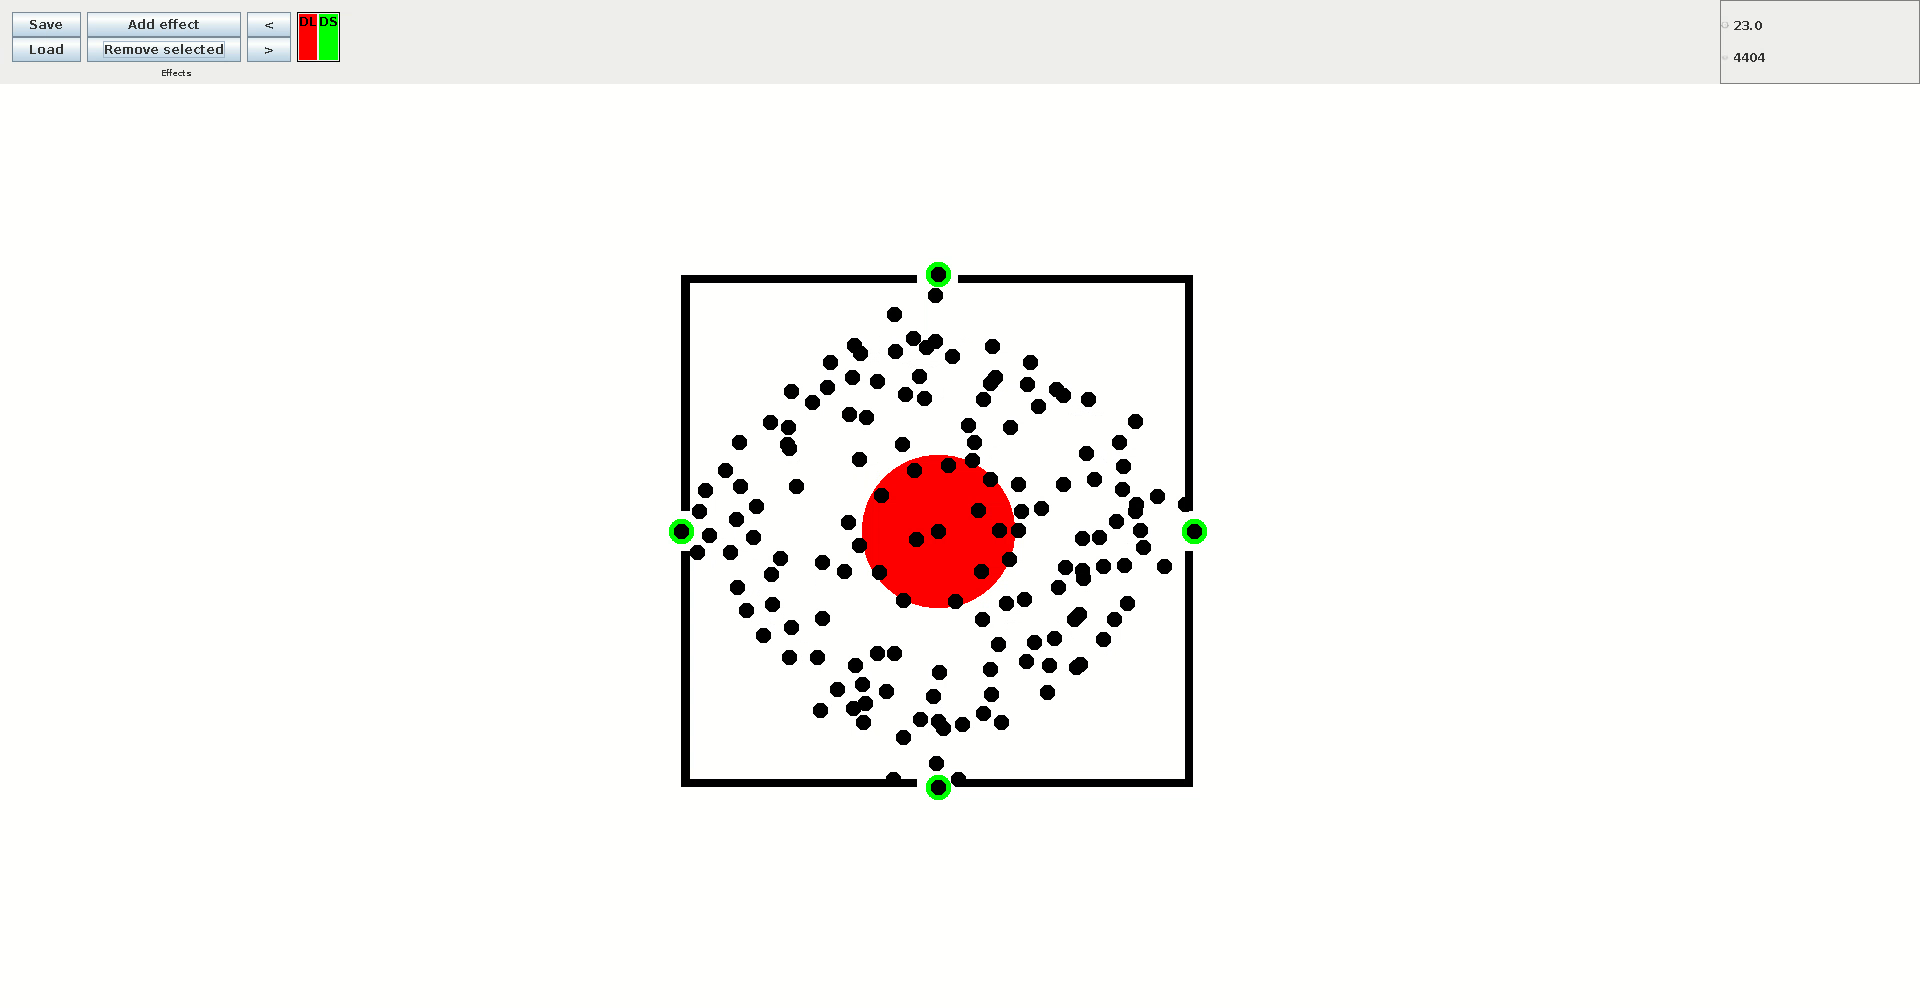
\includegraphics[width=\textwidth]{immagini/casi-studio/multiple-exits-blended-during.png}
    \end{subfigure}
    \hfill
    \begin{subfigure}[b]{0.75\textwidth}
        \centering
        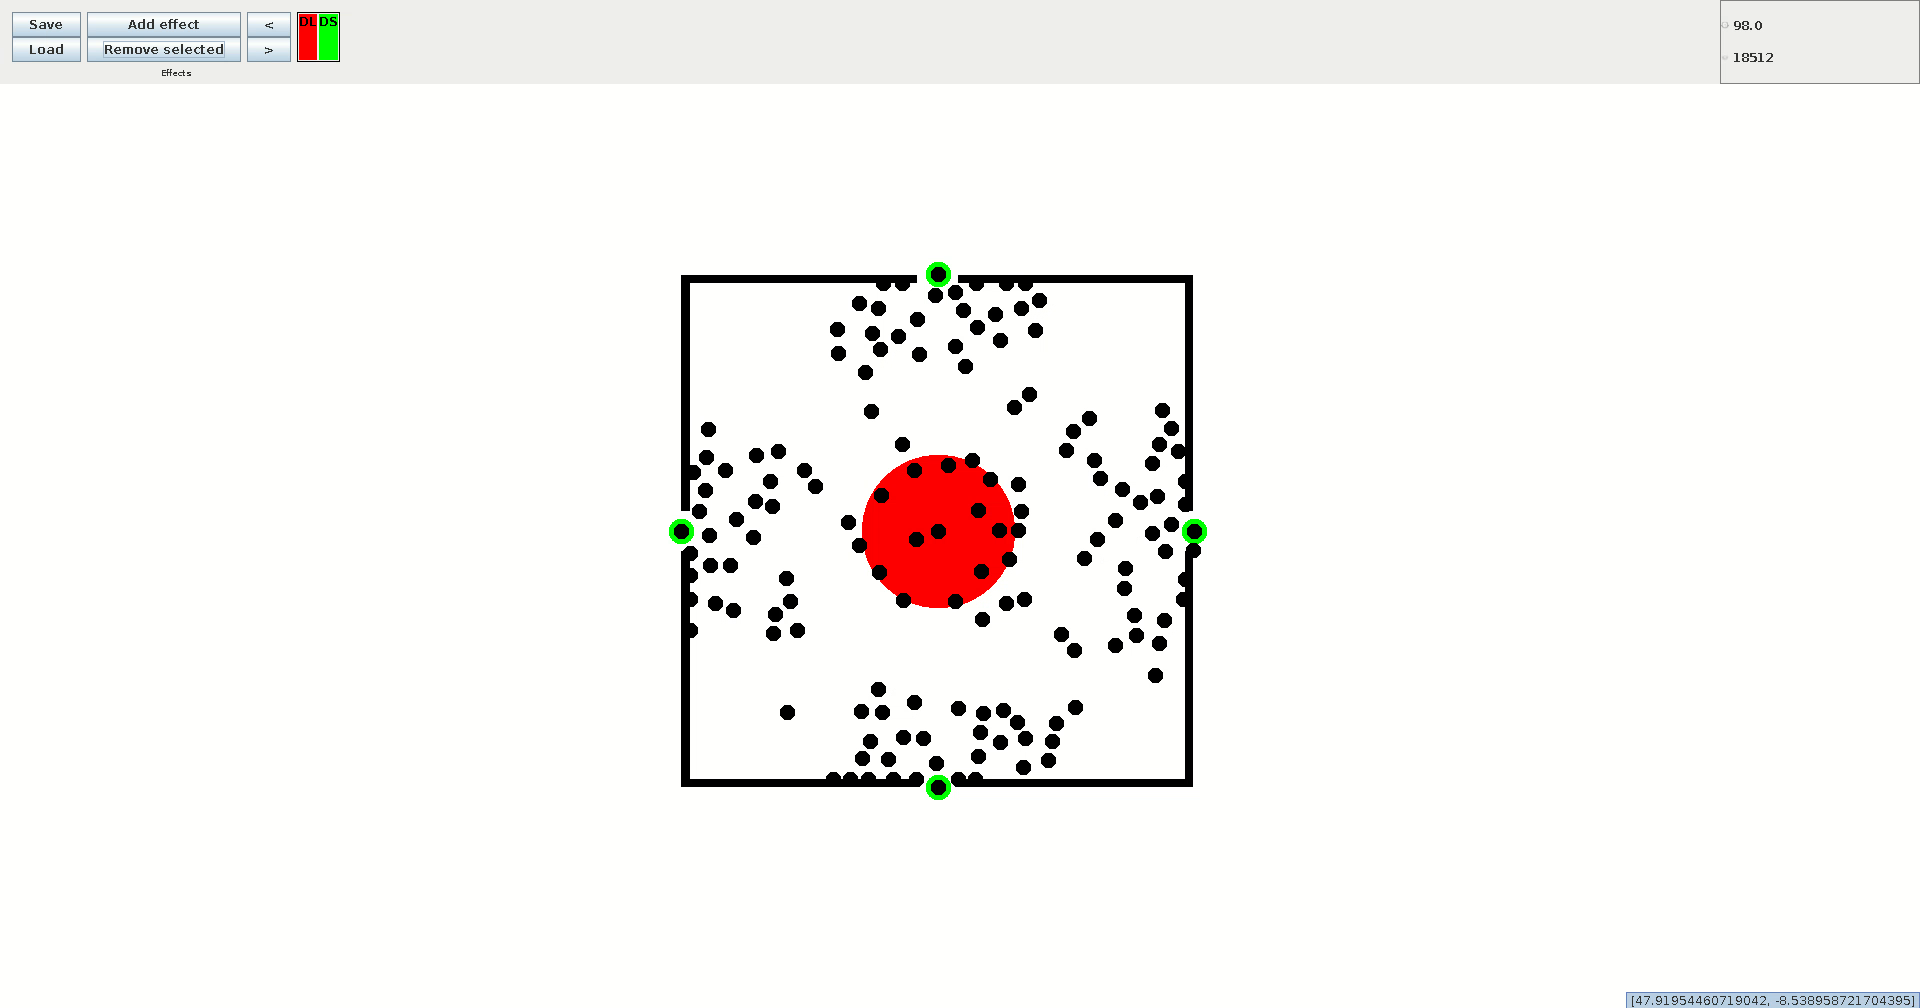
\includegraphics[width=\textwidth]{immagini/casi-studio/multiple-exits-blended-end.png}
    \end{subfigure}
    \caption{Fotogrammi salienti della simulazione sulla scelta dell'uscita utilizzando come strategia il \texttt{BlendedSteering}; le molteplici direzioni che il pedone è portato a seguire dai vari comportamenti di steering conducono a risultati inverosimili.}
    \label{fig:multiple-exits-blended}
\end{figure}

\begin{figure}
    \centering
    \begin{subfigure}[b]{0.75\textwidth}
        \centering
        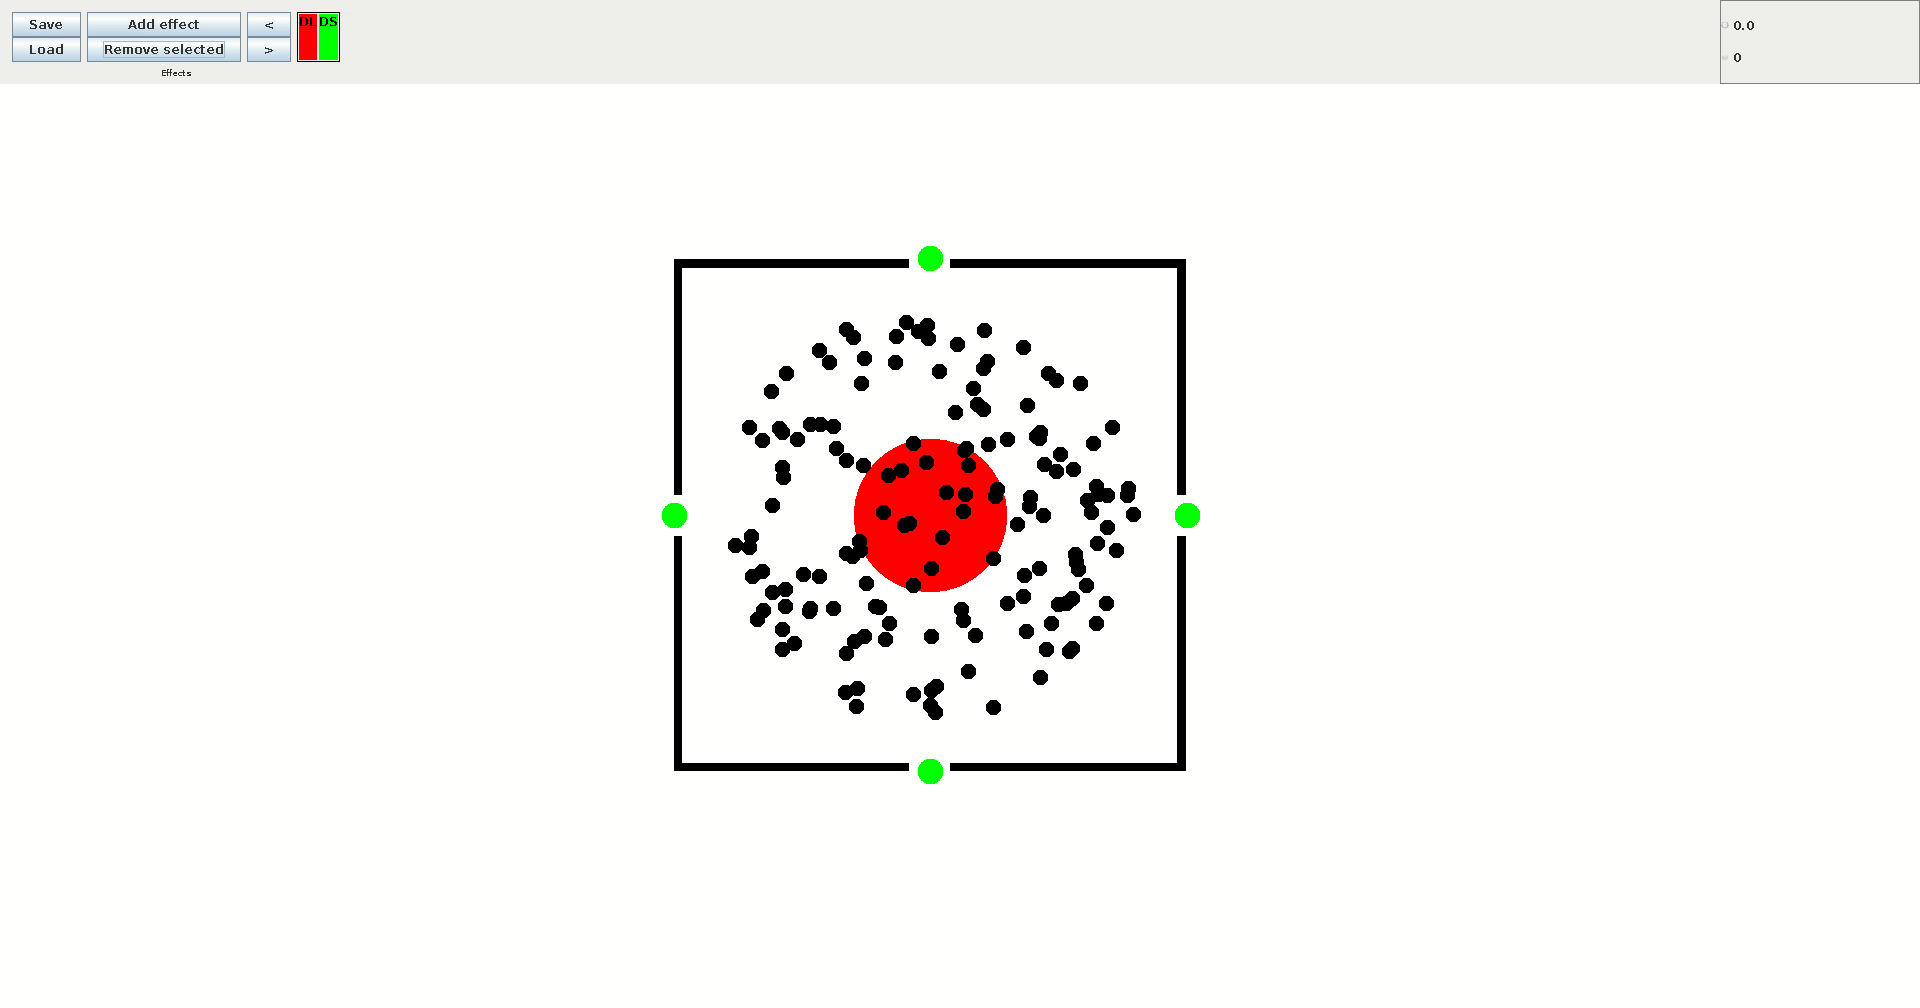
\includegraphics[width=\textwidth]{immagini/casi-studio/multiple-exits-priority-begin.png}
    \end{subfigure}
    \hfill
    \begin{subfigure}[b]{0.75\textwidth}
        \centering
        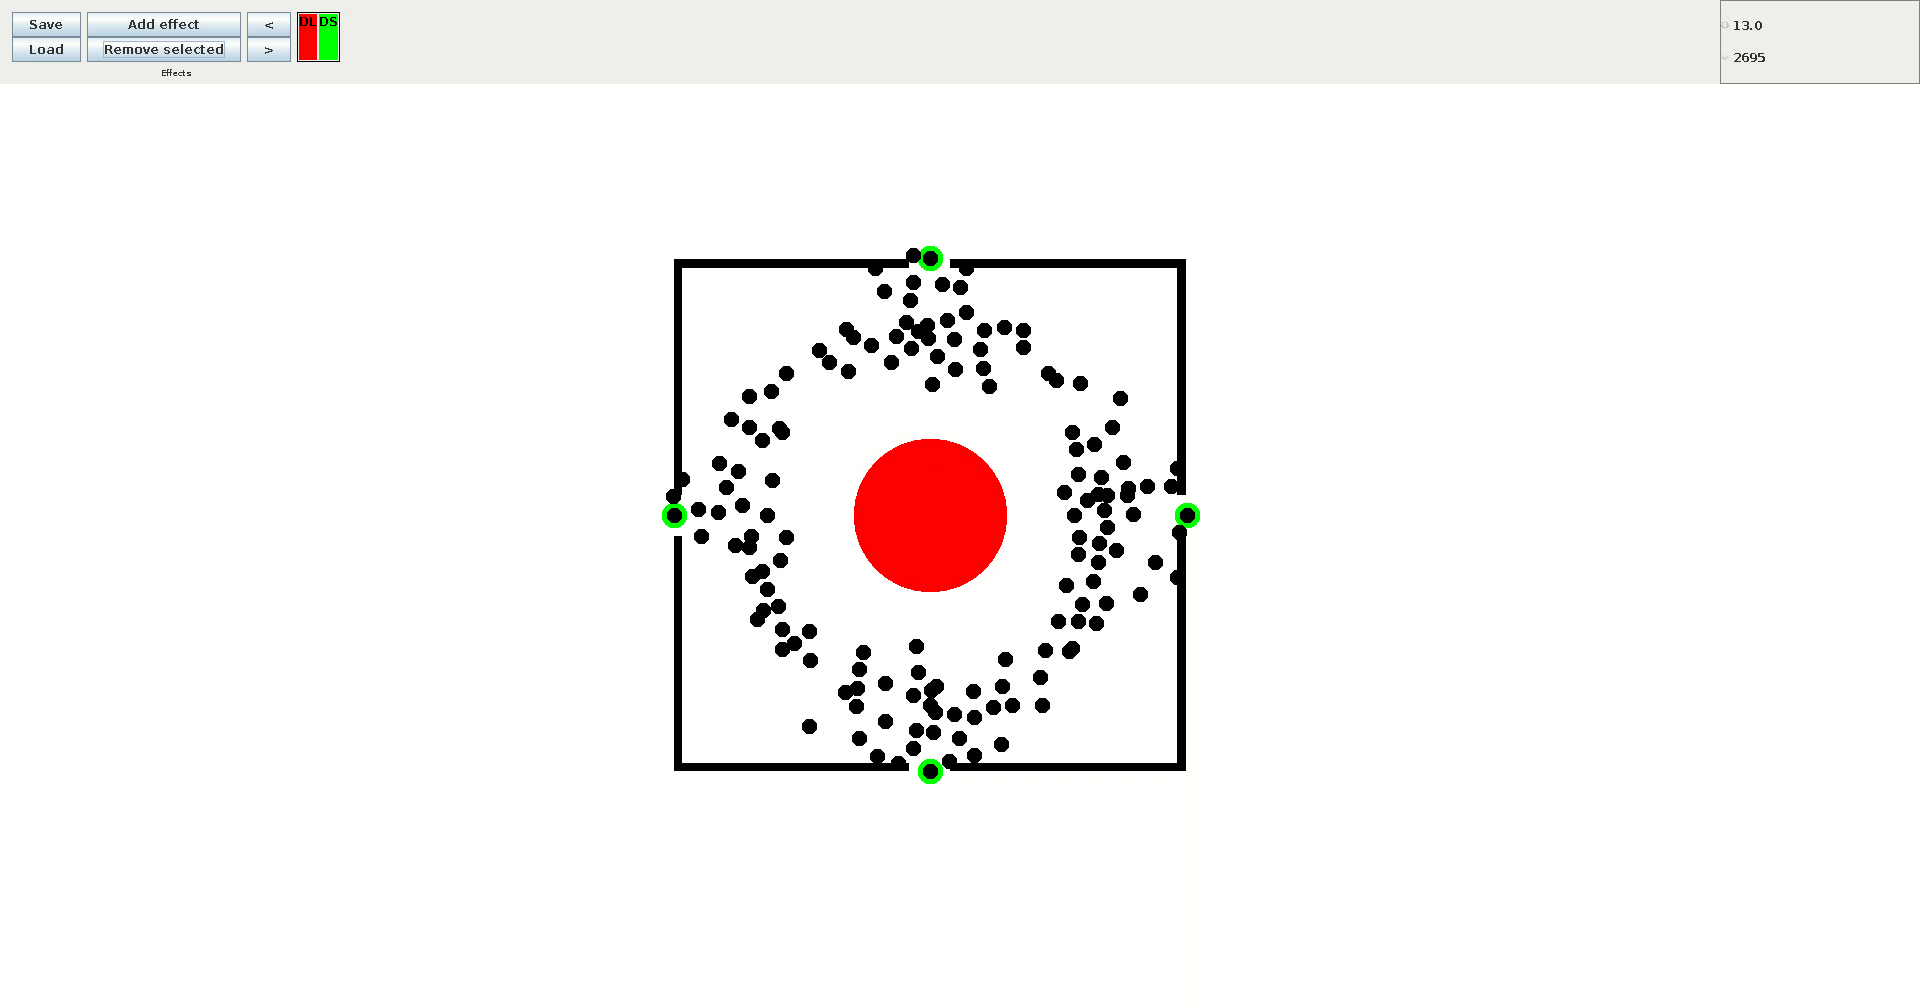
\includegraphics[width=\textwidth]{immagini/casi-studio/multiple-exits-priority-during.png}
    \end{subfigure}
    \hfill
    \begin{subfigure}[b]{0.75\textwidth}
        \centering
        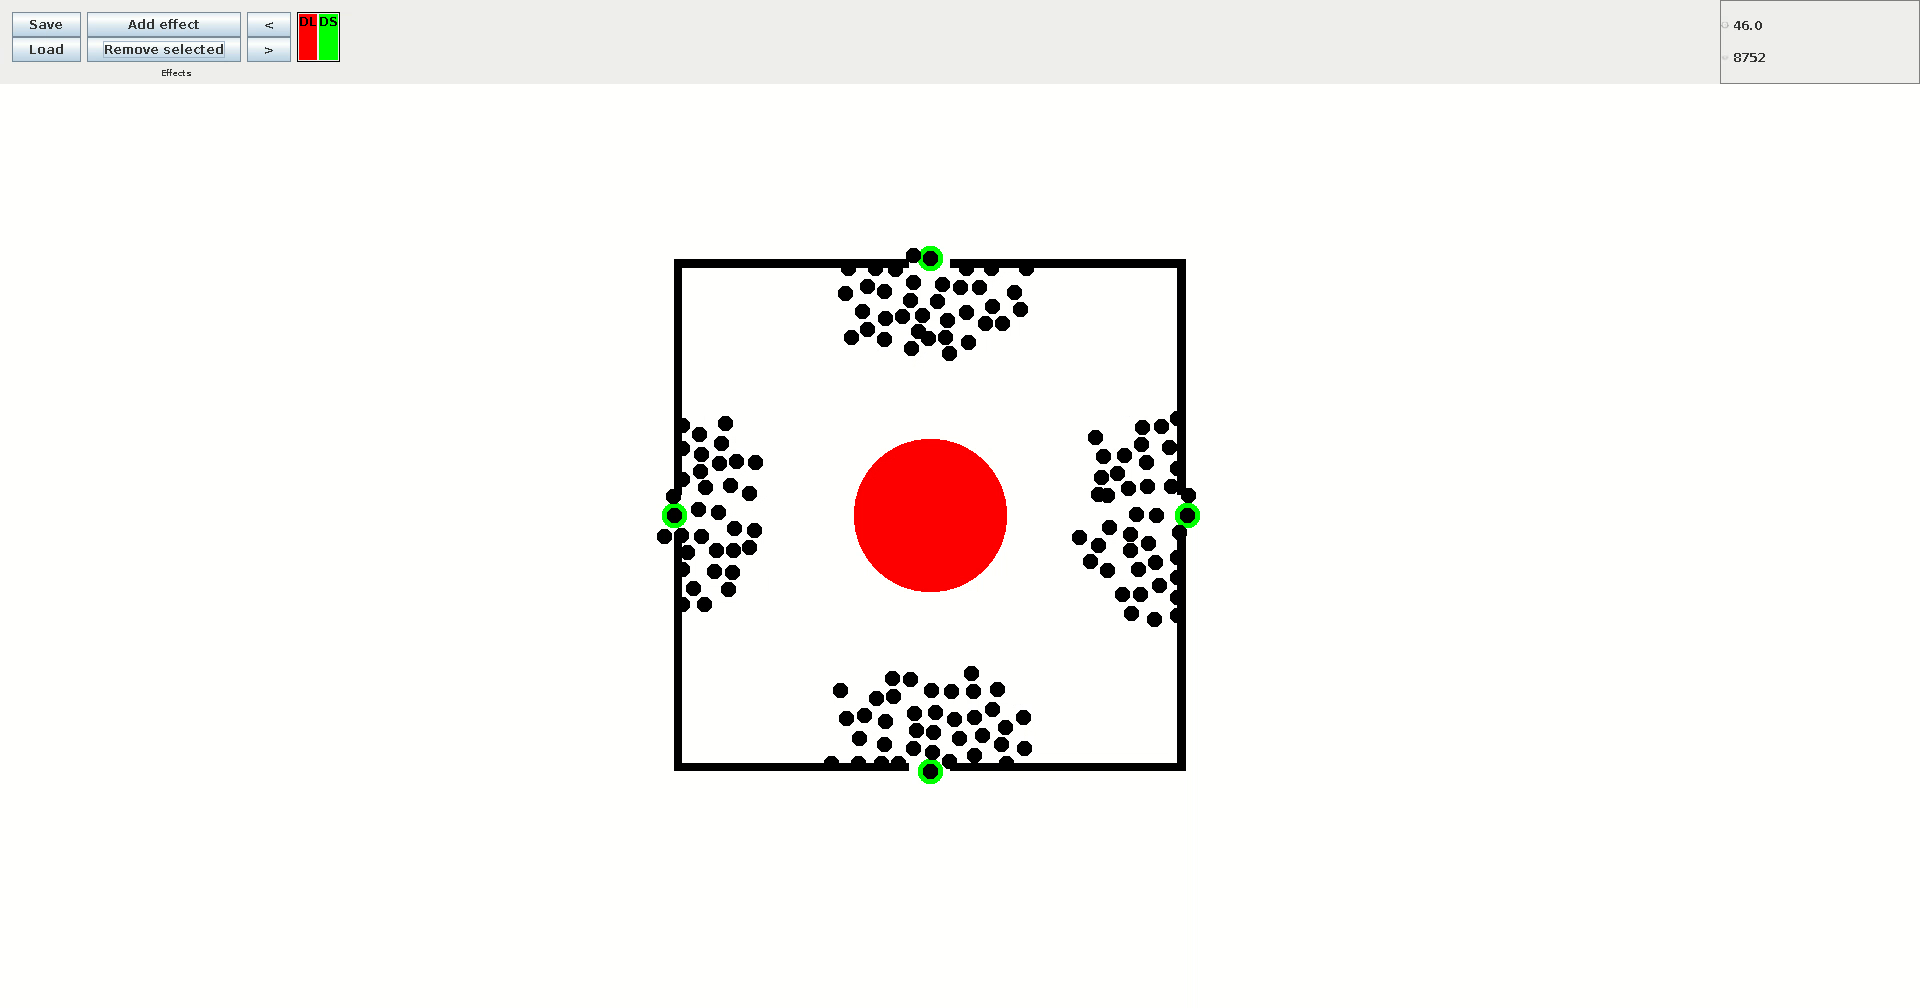
\includegraphics[width=\textwidth]{immagini/casi-studio/multiple-exits-priority-end.png}
    \end{subfigure}
    \caption{Fotogrammi salienti della simulazione sulla scelta dell'uscita utilizzando come strategia il \texttt{PrioritySteering}; definendo una priorità tra le azioni da eseguire, è possibile condurre i pedoni verso l'uscita loro più congeniale.}
    \label{fig:multiple-exits-priority}
\end{figure}
\section{Presenza di ostacoli}
Gli ambienti visti fino ad ora non presentano alcun tipo di ostacolo, quindi un nodo è vincolato nel movimento solo dalla presenza nelle sue vicinanze di eventuali altri suoi simili. \newline
Per descrivere in maniera più dettagliata uno scenario, è necessario considerare anche la presenza di oggetti al suo interno, che in relazione alla loro grandezza e alla loro posizione possono incidere significativamente sui tempi necessari ad un pedone per scappare o raggiungere una determinata zona.

\subsection{Descrizione della simulazione}
Grazie all'uso dell'\texttt{ImageEnvironment} è stato possibile definire un ambiente contenente cinque ostacoli: quattro rettangolari rispettivamente in alto, in basso, a destra e a sinistra della scena ed uno circolare al centro di essa. \newline
Si è pensato di collocare tre insiemi di pedoni nelle vicinanze di questi oggetti e di definire una zona di sicurezza comune, avendo cura che vi fosse almeno un elemento di intralcio tra essa ed un qualsiasi agente. \newline
La simulazione è stata eseguita prima non considerando il comportamento di steering dell'aggiramento degli ostacoli, poi inserendolo tra le azioni.

\subsection{Risultati ottenuti}
Mentre nella prima simulazione molti nodi rimangono attaccati agli ostacoli, nel vano tentativo di volerci passare attraverso per raggiungere la zona di loro interesse (figura \ref{fig:no-obstacle-avoidance}), nella seconda tutti i pedoni riescono ad arrivare a destinazione, schivando i vari oggetti nella direzione loro più congeniale in relazione alla posizione da cui erano partiti. Il tragitto percorso è deducibile dalla figura \ref{fig:obstacle-avoidance}.

\begin{figure}
    \centering
    \begin{subfigure}[b]{0.75\textwidth}
        \centering
        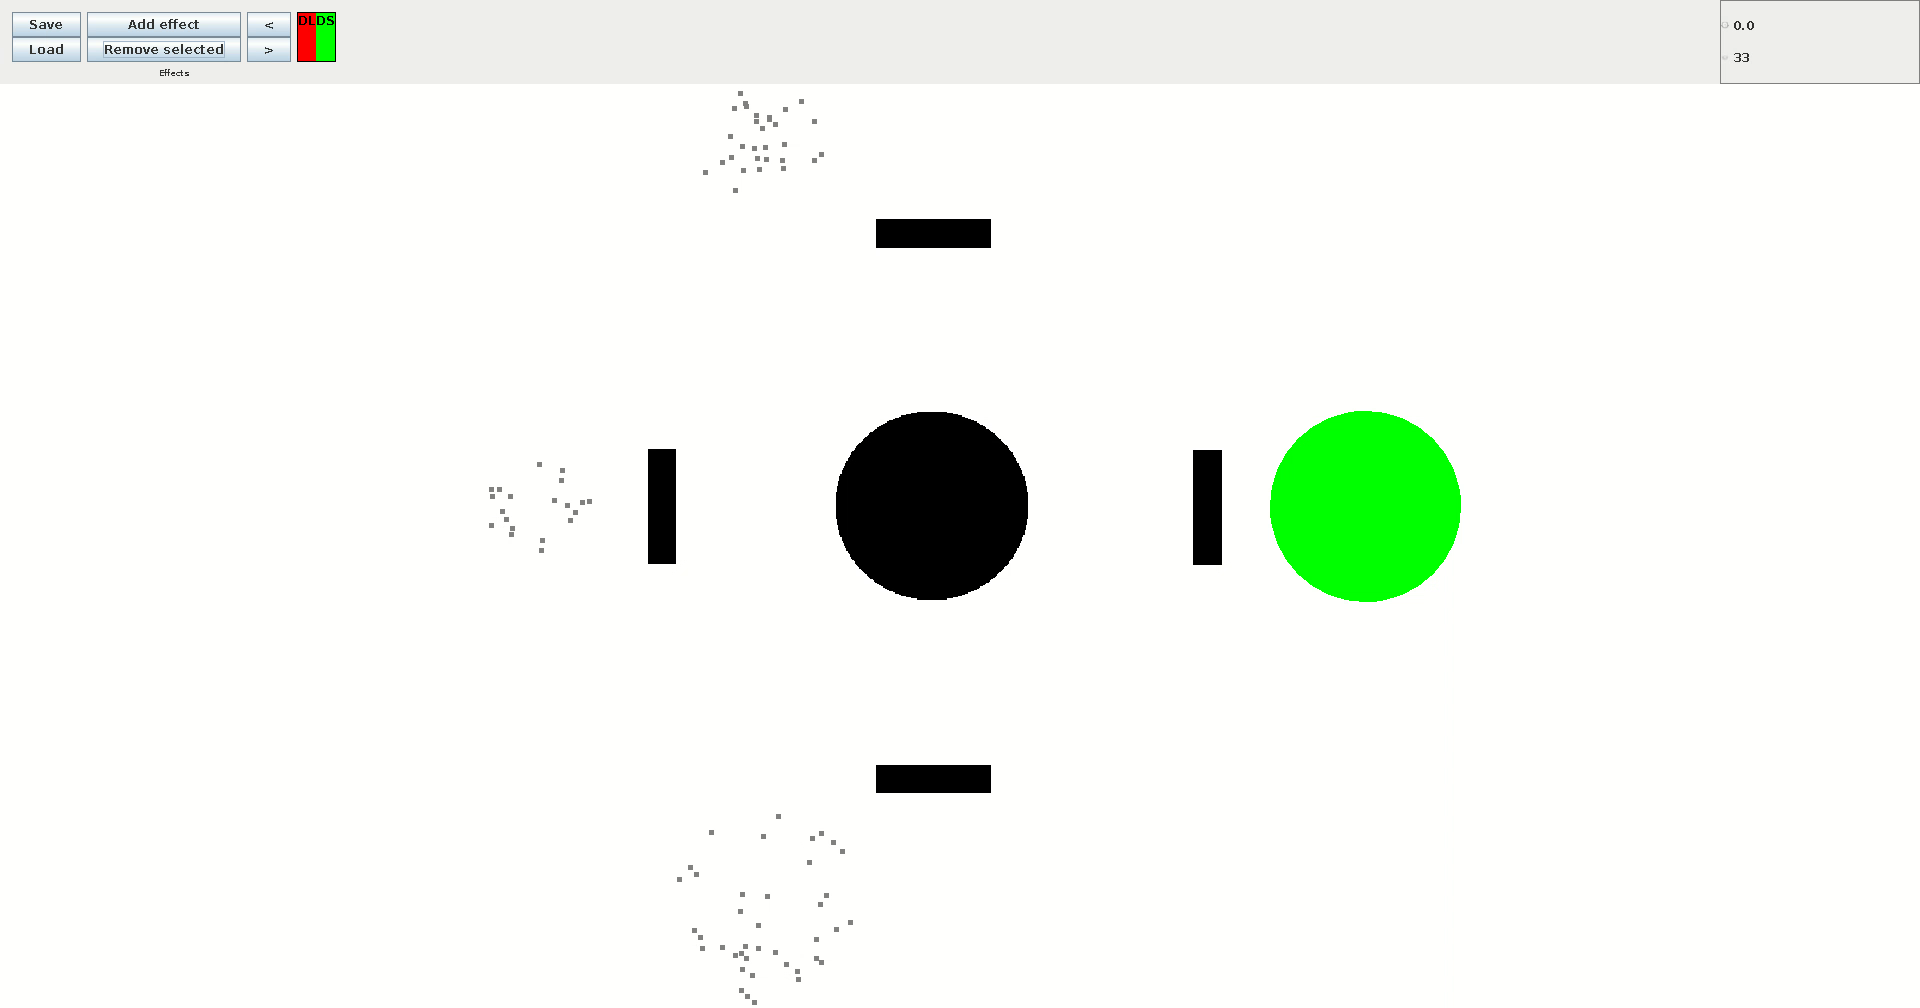
\includegraphics[width=\textwidth]{immagini/casi-studio/no-obstacle-avoidance-begin.png}
    \end{subfigure}
    \hfill
    \begin{subfigure}[b]{0.75\textwidth}
        \centering
        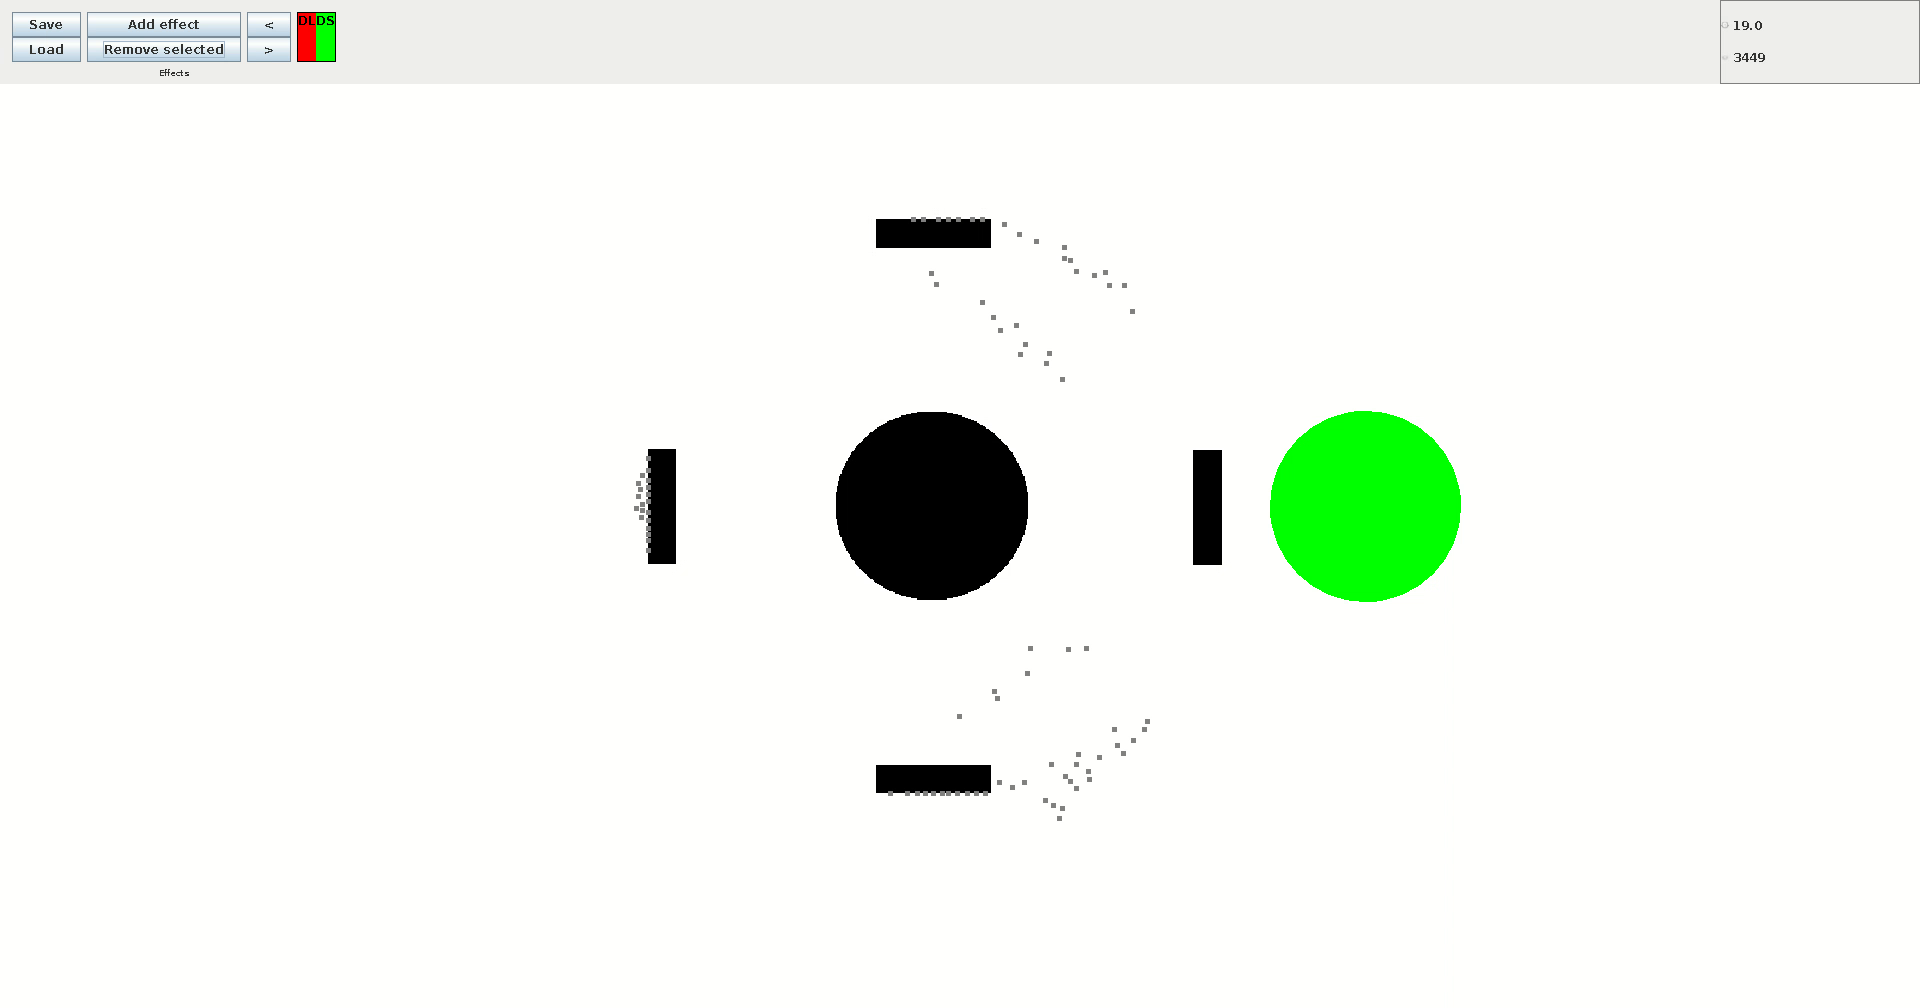
\includegraphics[width=\textwidth]{immagini/casi-studio/no-obstacle-avoidance-during.png}
    \end{subfigure}
    \hfill
    \begin{subfigure}[b]{0.75\textwidth}
        \centering
        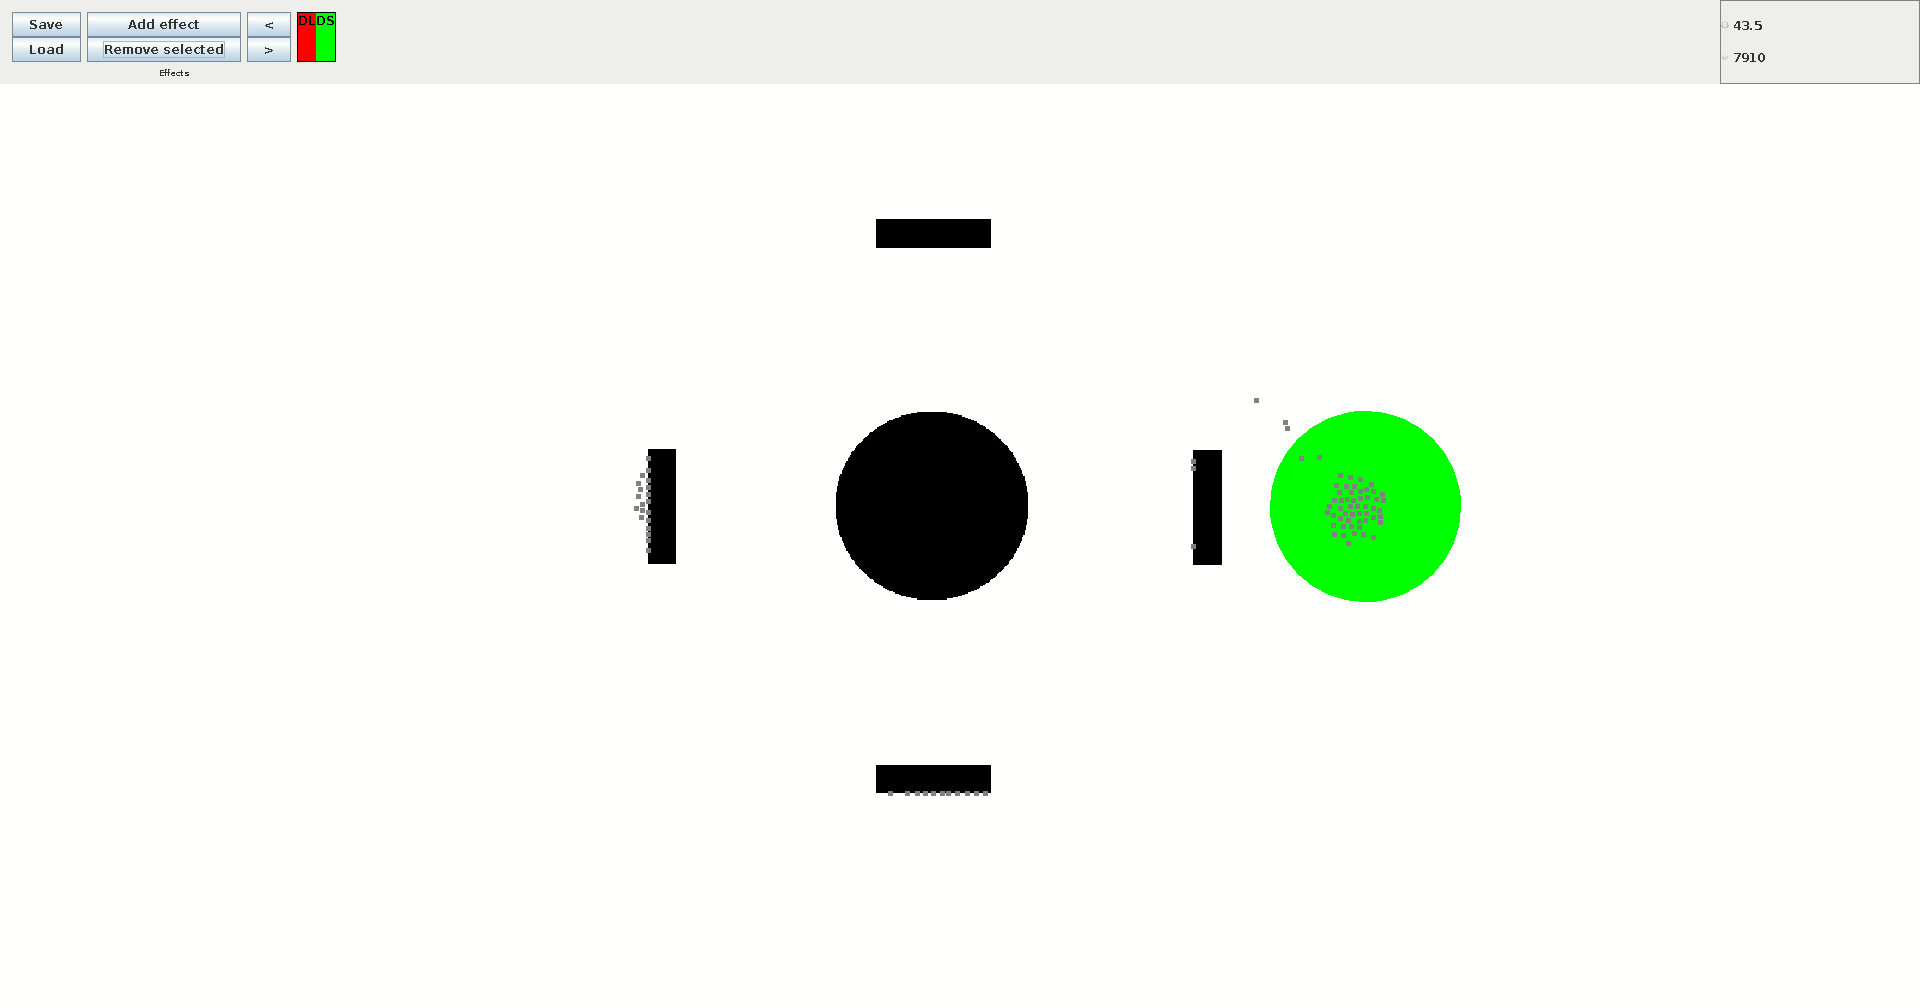
\includegraphics[width=\textwidth]{immagini/casi-studio/no-obstacle-avoidance-end.png}
    \end{subfigure}
    \caption{Fotogrammi salienti della simulazione in cui sono presenti ostacoli non considerando il comportamento di steering ad essi associato; molti pedoni rimangono bloccati durante il loro percorso e non riescono a raggiungere la zona di sicurezza.}
    \label{fig:no-obstacle-avoidance}
\end{figure}

\begin{figure}
    \centering
    \begin{subfigure}[b]{0.75\textwidth}
        \centering
        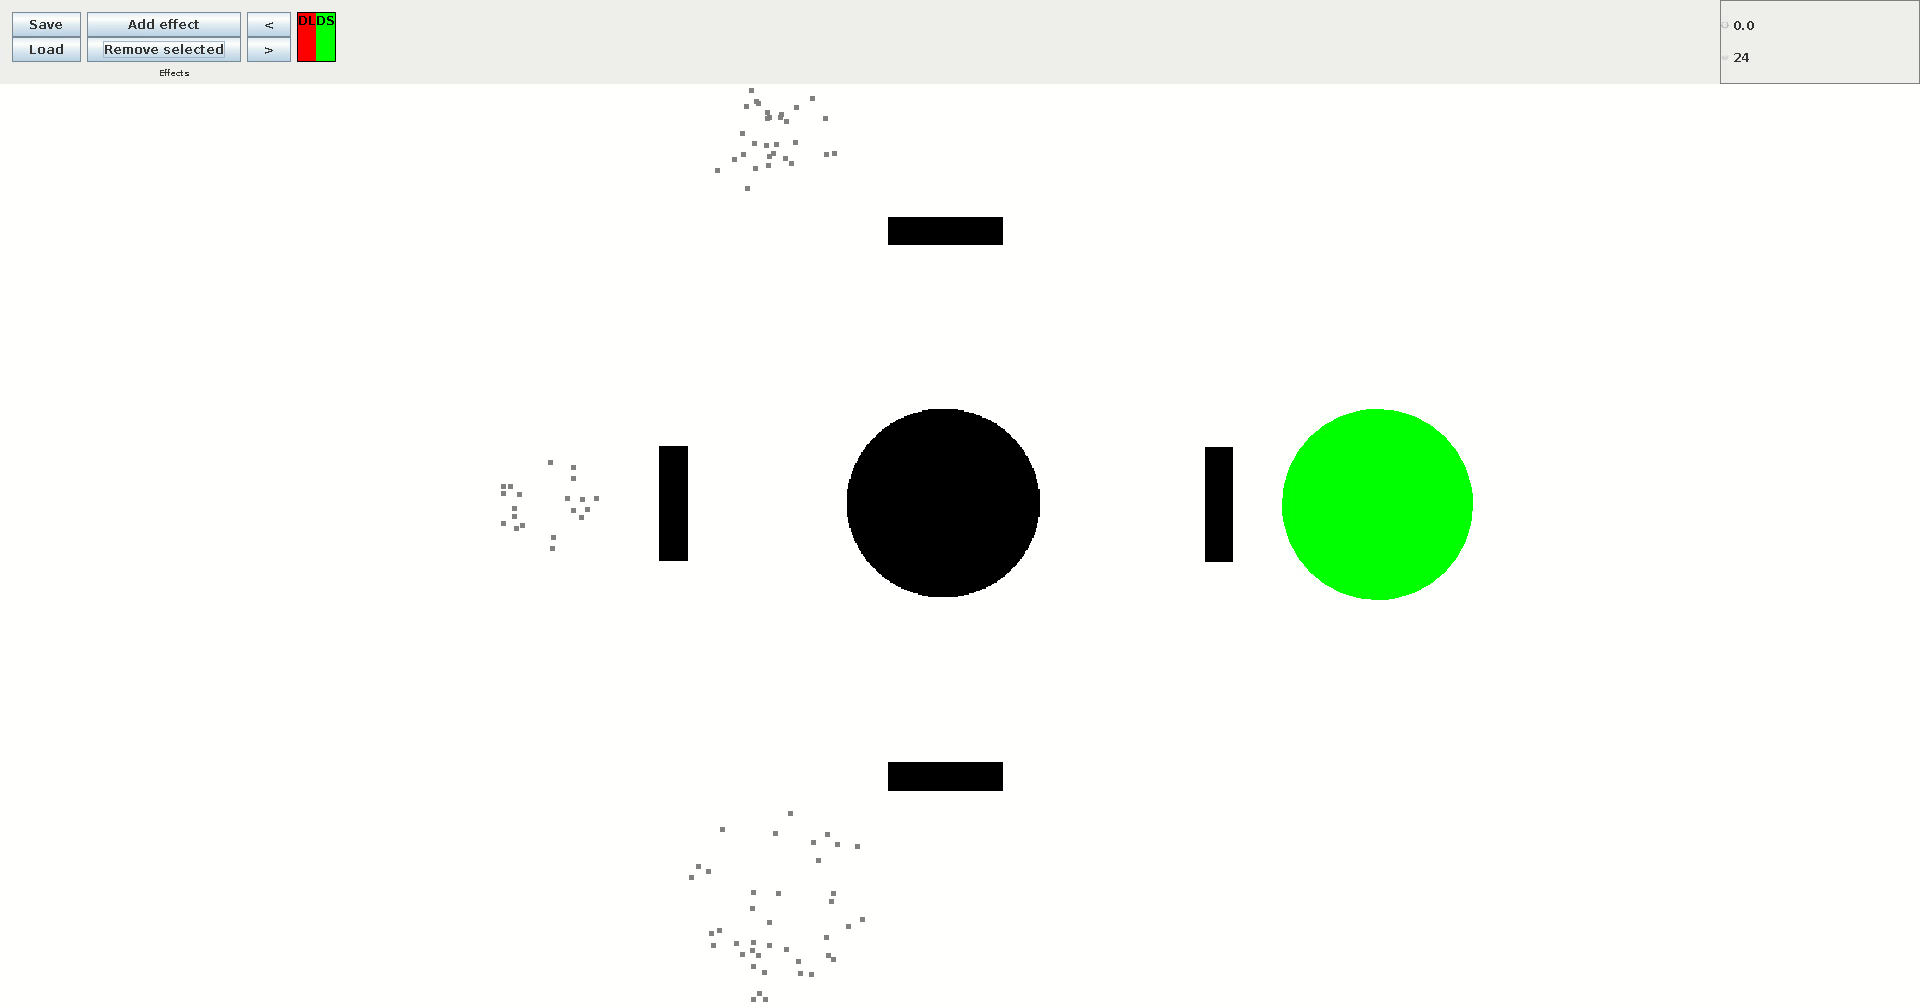
\includegraphics[width=\textwidth]{immagini/casi-studio/obstacle-avoidance-begin.png}
    \end{subfigure}
    \hfill
    \begin{subfigure}[b]{0.75\textwidth}
        \centering
        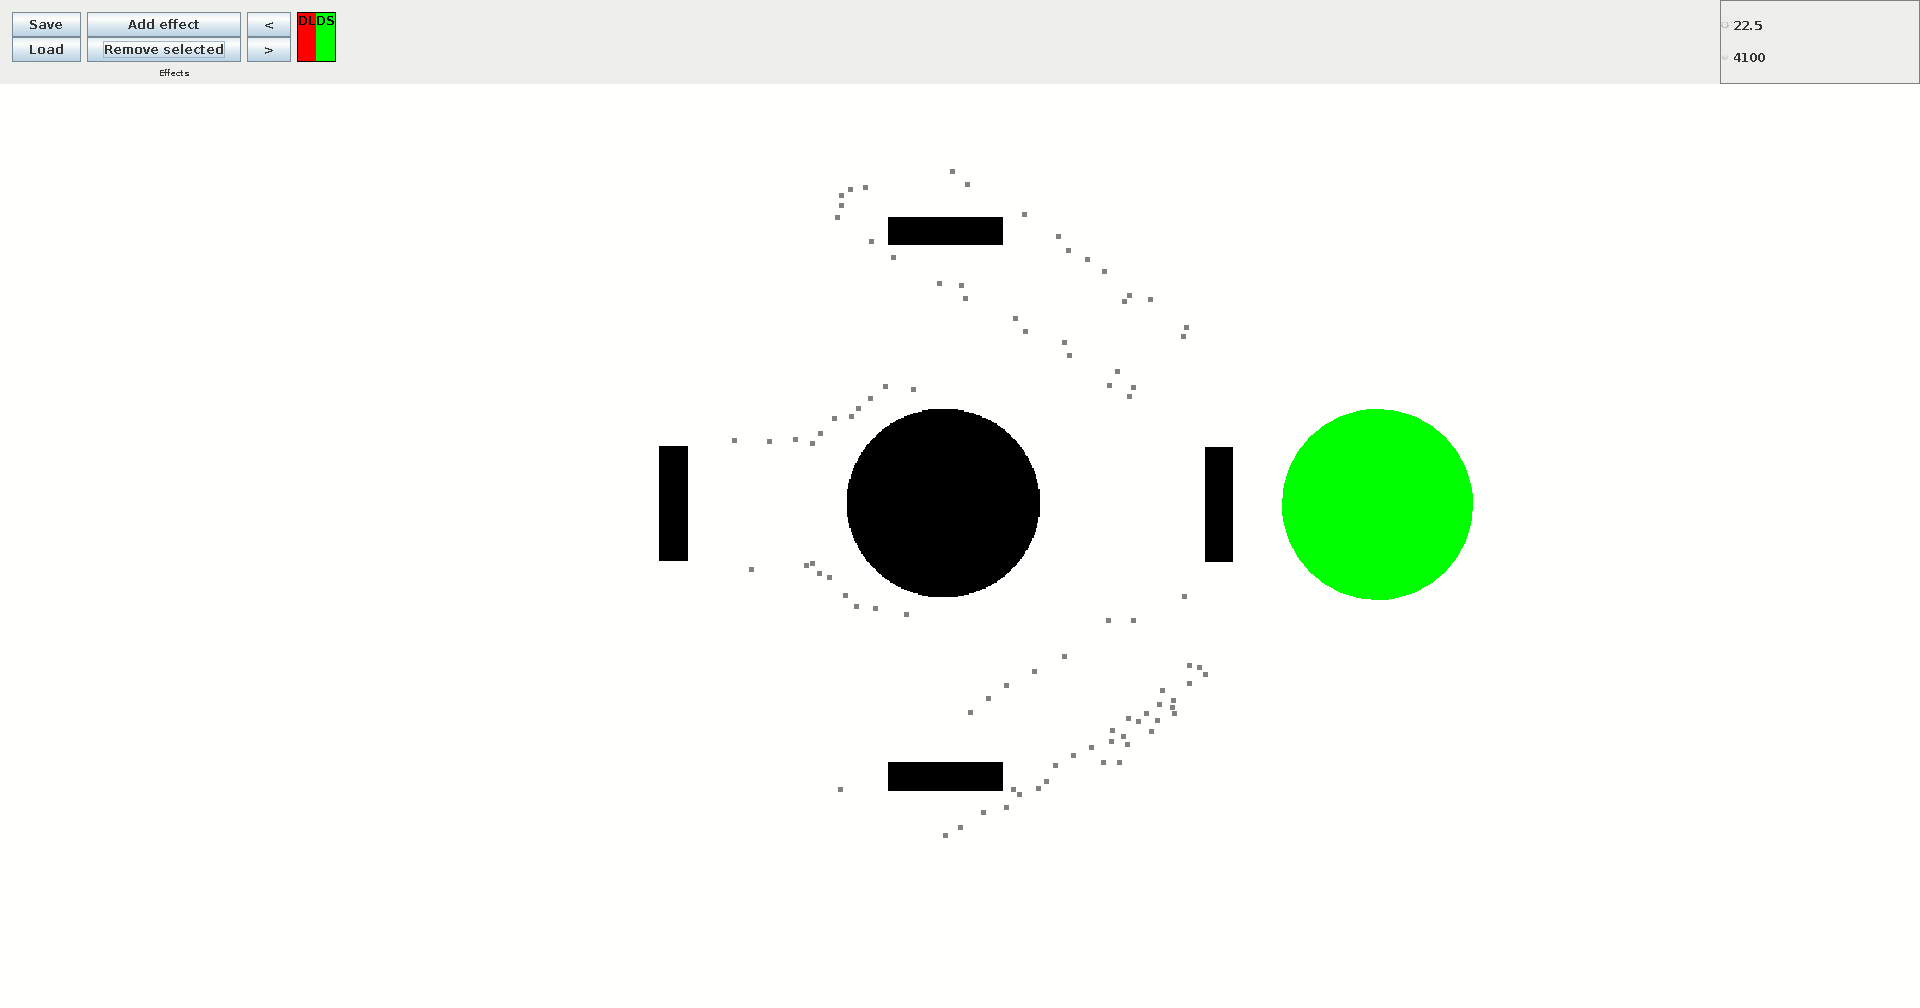
\includegraphics[width=\textwidth]{immagini/casi-studio/obstacle-avoidance-during.png}
    \end{subfigure}
    \hfill
    \begin{subfigure}[b]{0.75\textwidth}
        \centering
        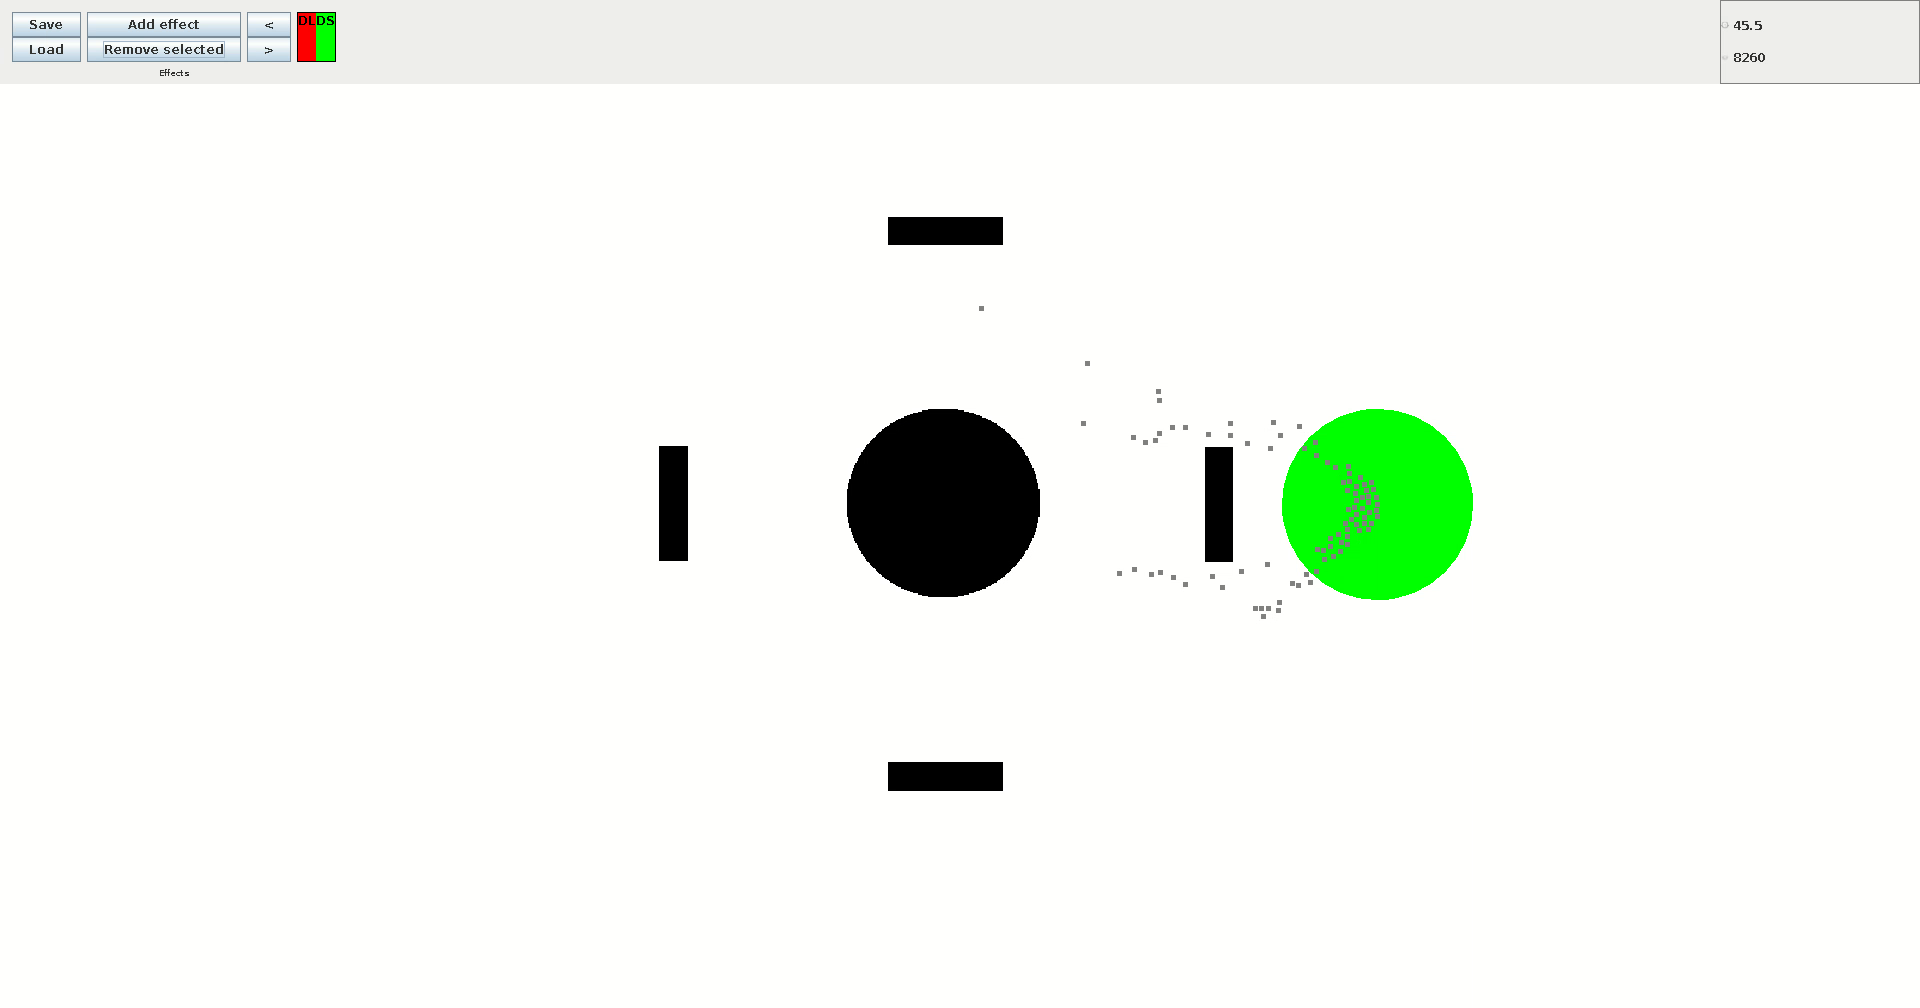
\includegraphics[width=\textwidth]{immagini/casi-studio/obstacle-avoidance-end.png}
    \end{subfigure}
    \caption{Fotogrammi salienti della simulazione in cui sono presenti ostacoli considerando il comportamento di steering ad essi associato; tutti i pedoni riescono a raggiungere la zona di sicurezza evitando eventuali oggetti presenti sul loro cammino.}
    \label{fig:obstacle-avoidance}
\end{figure}